% Options for packages loaded elsewhere
\PassOptionsToPackage{unicode}{hyperref}
\PassOptionsToPackage{hyphens}{url}
\documentclass[
  12pt,
]{article}
\usepackage{xcolor}
\usepackage[margin=1in]{geometry}
\usepackage{amsmath,amssymb}
\setcounter{secnumdepth}{-\maxdimen} % remove section numbering
\usepackage{iftex}
\ifPDFTeX
  \usepackage[T1]{fontenc}
  \usepackage[utf8]{inputenc}
  \usepackage{textcomp} % provide euro and other symbols
\else % if luatex or xetex
  \usepackage{unicode-math} % this also loads fontspec
  \defaultfontfeatures{Scale=MatchLowercase}
  \defaultfontfeatures[\rmfamily]{Ligatures=TeX,Scale=1}
\fi
\usepackage{lmodern}
\ifPDFTeX\else
  % xetex/luatex font selection
\fi
% Use upquote if available, for straight quotes in verbatim environments
\IfFileExists{upquote.sty}{\usepackage{upquote}}{}
\IfFileExists{microtype.sty}{% use microtype if available
  \usepackage[]{microtype}
  \UseMicrotypeSet[protrusion]{basicmath} % disable protrusion for tt fonts
}{}
\makeatletter
\@ifundefined{KOMAClassName}{% if non-KOMA class
  \IfFileExists{parskip.sty}{%
    \usepackage{parskip}
  }{% else
    \setlength{\parindent}{0pt}
    \setlength{\parskip}{6pt plus 2pt minus 1pt}}
}{% if KOMA class
  \KOMAoptions{parskip=half}}
\makeatother
\usepackage{color}
\usepackage{fancyvrb}
\newcommand{\VerbBar}{|}
\newcommand{\VERB}{\Verb[commandchars=\\\{\}]}
\DefineVerbatimEnvironment{Highlighting}{Verbatim}{commandchars=\\\{\}}
% Add ',fontsize=\small' for more characters per line
\usepackage{framed}
\definecolor{shadecolor}{RGB}{248,248,248}
\newenvironment{Shaded}{\begin{snugshade}}{\end{snugshade}}
\newcommand{\AlertTok}[1]{\textcolor[rgb]{0.94,0.16,0.16}{#1}}
\newcommand{\AnnotationTok}[1]{\textcolor[rgb]{0.56,0.35,0.01}{\textbf{\textit{#1}}}}
\newcommand{\AttributeTok}[1]{\textcolor[rgb]{0.13,0.29,0.53}{#1}}
\newcommand{\BaseNTok}[1]{\textcolor[rgb]{0.00,0.00,0.81}{#1}}
\newcommand{\BuiltInTok}[1]{#1}
\newcommand{\CharTok}[1]{\textcolor[rgb]{0.31,0.60,0.02}{#1}}
\newcommand{\CommentTok}[1]{\textcolor[rgb]{0.56,0.35,0.01}{\textit{#1}}}
\newcommand{\CommentVarTok}[1]{\textcolor[rgb]{0.56,0.35,0.01}{\textbf{\textit{#1}}}}
\newcommand{\ConstantTok}[1]{\textcolor[rgb]{0.56,0.35,0.01}{#1}}
\newcommand{\ControlFlowTok}[1]{\textcolor[rgb]{0.13,0.29,0.53}{\textbf{#1}}}
\newcommand{\DataTypeTok}[1]{\textcolor[rgb]{0.13,0.29,0.53}{#1}}
\newcommand{\DecValTok}[1]{\textcolor[rgb]{0.00,0.00,0.81}{#1}}
\newcommand{\DocumentationTok}[1]{\textcolor[rgb]{0.56,0.35,0.01}{\textbf{\textit{#1}}}}
\newcommand{\ErrorTok}[1]{\textcolor[rgb]{0.64,0.00,0.00}{\textbf{#1}}}
\newcommand{\ExtensionTok}[1]{#1}
\newcommand{\FloatTok}[1]{\textcolor[rgb]{0.00,0.00,0.81}{#1}}
\newcommand{\FunctionTok}[1]{\textcolor[rgb]{0.13,0.29,0.53}{\textbf{#1}}}
\newcommand{\ImportTok}[1]{#1}
\newcommand{\InformationTok}[1]{\textcolor[rgb]{0.56,0.35,0.01}{\textbf{\textit{#1}}}}
\newcommand{\KeywordTok}[1]{\textcolor[rgb]{0.13,0.29,0.53}{\textbf{#1}}}
\newcommand{\NormalTok}[1]{#1}
\newcommand{\OperatorTok}[1]{\textcolor[rgb]{0.81,0.36,0.00}{\textbf{#1}}}
\newcommand{\OtherTok}[1]{\textcolor[rgb]{0.56,0.35,0.01}{#1}}
\newcommand{\PreprocessorTok}[1]{\textcolor[rgb]{0.56,0.35,0.01}{\textit{#1}}}
\newcommand{\RegionMarkerTok}[1]{#1}
\newcommand{\SpecialCharTok}[1]{\textcolor[rgb]{0.81,0.36,0.00}{\textbf{#1}}}
\newcommand{\SpecialStringTok}[1]{\textcolor[rgb]{0.31,0.60,0.02}{#1}}
\newcommand{\StringTok}[1]{\textcolor[rgb]{0.31,0.60,0.02}{#1}}
\newcommand{\VariableTok}[1]{\textcolor[rgb]{0.00,0.00,0.00}{#1}}
\newcommand{\VerbatimStringTok}[1]{\textcolor[rgb]{0.31,0.60,0.02}{#1}}
\newcommand{\WarningTok}[1]{\textcolor[rgb]{0.56,0.35,0.01}{\textbf{\textit{#1}}}}
\usepackage{graphicx}
\makeatletter
\newsavebox\pandoc@box
\newcommand*\pandocbounded[1]{% scales image to fit in text height/width
  \sbox\pandoc@box{#1}%
  \Gscale@div\@tempa{\textheight}{\dimexpr\ht\pandoc@box+\dp\pandoc@box\relax}%
  \Gscale@div\@tempb{\linewidth}{\wd\pandoc@box}%
  \ifdim\@tempb\p@<\@tempa\p@\let\@tempa\@tempb\fi% select the smaller of both
  \ifdim\@tempa\p@<\p@\scalebox{\@tempa}{\usebox\pandoc@box}%
  \else\usebox{\pandoc@box}%
  \fi%
}
% Set default figure placement to htbp
\def\fps@figure{htbp}
\makeatother
\setlength{\emergencystretch}{3em} % prevent overfull lines
\providecommand{\tightlist}{%
  \setlength{\itemsep}{0pt}\setlength{\parskip}{0pt}}
\usepackage{fontspec}
\usepackage{indentfirst}
\usepackage{setspace}
\usepackage{fvextra}
\fvset{breaklines=true,breakanywhere=true}
\setmainfont{Times New Roman}
\setlength{\parindent}{1.18cm}
\setstretch{1.5}
\usepackage{bookmark}
\IfFileExists{xurl.sty}{\usepackage{xurl}}{} % add URL line breaks if available
\urlstyle{same}
\hypersetup{
  hidelinks,
  pdfcreator={LaTeX via pandoc}}

\author{}
\date{\vspace{-2.5em}}

\begin{document}

\begin{center}

\vspace*{1cm}

{\Large \textbf{ANALISIS DATA PEMBANGUNAN WILAYAH}}

\vspace{0.3cm}

{\Large \textbf{MENGGUNAKAN R}}

\vspace{2cm}

\textbf{Disusun Oleh:}

\vspace{0.8cm}

\begin{tabular}{p{8cm}p{3cm}}
Diaz Ramaananta Harahap & J0403251048\\
Nashira Salima Firmansyah & J0403251056\\
Dede Risma Komalasari & J0403251049\\
Zalfa Nazla Azkiya & J0403251037\\
Fahrizal Azis & J0403251151\\
Muhamad Akbar Zainuri & J0403251008\\
\end{tabular}

\vspace{1.2cm}


\includegraphics[width=3.5cm]{../gambar/Logo_IPB.png}

\vspace{1.5cm}

\textbf{MATA KULIAH PROBABILITAS \& STATISTIKA}

\vspace{0.3cm}

\textbf{PROGRAM STUDI TEKNOLOGI REKAYASA PERANGKAT LUNAK}

\vspace{0.3cm}

\textbf{SEKOLAH VOKASI}

\vspace{0.3cm}

\textbf{INSTITUT PERTANIAN BOGOR}

\vspace{1.5cm}

\textbf{2026}

\end{center}

\newpage

\thispagestyle{empty}

\newpage

\begin{center}
  {
    \bfseries

    \vfill

    \Large

    BAB I

    PENDAHULUAN
  }
\end{center}

\subsection{\texorpdfstring{\normalsize 1.1 \hspace {0,5cm} Latar
Belakang}{1.1  Latar Belakang}}\label{latar-belakang}

Pembangunan wilayah adalah sebuah proses yang bertujuan untuk
meningkatkan kesejahteraan masyarakat. Untuk mengetahui bagaimana suatu
pembangunan wilayah di suatu daerah berhasil diperlukan indikator yang
dapat menggambarkan keadaan masyarakat di wilayah tersebut dengan jelas,
seperti angka kemiskinan, pengangguran, Produk Domestik Regional Bruto
(PDRB), serta indeks pembangunan Manusia (IPM).

Oleh karena itu, diperlukan analisis data untuk mengolah informasi yang
ada agar dapat memberikan gambaran tentang kondisi pembangunan di suatu
wilayah. Berdasarkan kebutuhan tersebut, projek ini bertujuan untuk
menganalisis data pembangunan wilayah di seluruh Indonesia dengan
mengimplementasikan bahasa pemrograman R. Melalui projek akhir ini,
mahasiswa diharapkan dapat meningkatkan keterampilan mereka dalam
mengolah, menganalisis, dan menginterpretasikan data terkait pembangunan
daerah dengan memanfaatkan bahasa pemrograman R.

\subsection{\texorpdfstring{\normalsize 1.2 \hspace {0,5cm}
Tujuan}{1.2  Tujuan}}\label{tujuan}

Proyek ini bertujuan untuk menganalisis data mengenai pembangunan
wilayah di Indonesia dengan memanfaatkan bahasa pemrograman R. Analisis
dilakukan untuk mengenali ciri-ciri data, memahami hubungan di antara
indikator pembangunan, serta mengungkap faktor-faktor yang memengaruhi
tingkat perkembangan suatu daerah. Di samping itu, proyek ini bertujuan
untuk mengaplikasikan konsep statistika dan analisis data dalam
menyelesaikan masalah yang ada serta menyajikan hasil analisis dengan
cara yang terstruktur dan informatif.

\setcounter{page}{1}

\newpage

\begin{center}
  {
    \bfseries
    
    \vfill
    
    \Large
    
    BAB II
    
    METODOLOGI
  }
\end{center}

\subsection{\texorpdfstring{\normalsize 2.1 \hspace {0,5cm}
Dataset}{2.1  Dataset}}\label{dataset}

Dataset adalah kumpulan data terstruktur yang digunakan untuk berbagai
keperluan, seperti analisis, penelitian, atau pengolahan informasi
lainnya. Di dalam sebuah dataset, terdapat sejumlah variabel yang
disusun dalam bentuk tabel. Setiap kolom mewakili atribut tertentu,
sementara setiap baris menggambarkan entitas atau observasi yang
berbeda. Dataset menjadi komponen penting dalam pengolahan data,
membantu menghasilkan informasi yang lebih bermakna dan bermanfaat.

Data yang digunakan dalam analisis ini adalah dataset skor pembangunan
wilayah tingkat Kabupaten/Kota di Indonesia. Secara keseluruhan, dataset
ini mencakup observasi 2.500 baris kabupaten/kota dengan 13 kolom
variabel, yang berada dalam rentang waktu lima tahun, yaitu dari tahun
2020 hingga 2024. Berikut adalah rincian variabel-variabel yang telah
dikelompokkan menjadi beberapa kategori:

\begin{enumerate}
\def\labelenumi{\arabic{enumi}.}
\tightlist
\item
  Variabel Identitas Data : wilayah, provinsi, dan tahun.
\item
  Variabel Ekonomi : pdrb\_perkapita, kemiskinan, dan pengangguran.
\item
  Variabel Pembangunan Manusia : ipm, harapan\_hidup,
  rata\_lama\_sekolah.
\item
  Variabel Infrastruktur : akses\_internet, jalan\_baik, air\_bersih.
\item
  Variabel Metadata : catatan\_data.
\end{enumerate}

Dataset pembangunan wilayah tersebut berbentuk dokumen .csv. Dokumen ini
bisa diunduh melalui
\url{https://pembangunanwilayahmissingoutlier.tiiny.site} untuk melihat
dataset secara keseluruhan.

\subsection{\texorpdfstring{\normalsize 2.2 \hspace {0,5cm} Tools Yang
Digunakan}{2.2  Tools Yang Digunakan}}\label{tools-yang-digunakan}

Dalam melakukan analisis data ini, digunakan perangkat lunak Rstudio dan
library ggplot2 untuk menghasilkan informasi yang terstruktur dan akurat
tentang pembangunan wilayah di Indonesia. Berikut adalah rincian tools
yang digunakan:

\begin{enumerate}
\def\labelenumi{\arabic{enumi}.}
\tightlist
\item
  \textbf{Dataset format .csv:} Digunakan sebagai format penyimpanan
  data mentah yang menjadi objek utama analisis.
\item
  \textbf{Bahasa Pemrograman R:} R digunakan sebagai bahasa pemrograman
  utama untuk komputasi statistik dan analisis data. Bahasa ini dipilih
  karena memiliki kemampuan yang kuat dalam melakukan manipulasi data,
  serta menyediakan berbagai paket statistik yang mumpuni untuk
  melakukan analisis deskriptif maupun inferensial pada dataset.
\item
  \textbf{RStudio:} RStudio digunakan sebagai \emph{Integrated
  Development Environment} (IDE) atau lingkungan pengembangan
  terintegrasi untuk menulis dan mengeksekusi kode R. RStudio
  mempermudah manajemen proyek, pemantauan variabel, penanganan error
  melalui antarmuka yang interaktif, serta mendukung penyusunan laporan
  menggunakan R Markdown.
\item
  \textbf{Library ggplot2:} Library ggplot2 digunakan untuk memenuhi
  kebutuhan visualisasi data. Library ini memungkinkan pembuatan grafik
  secara modular. Di dalam proyek ini, ggplot2 digunakan untuk
  menyajikan tren indikator pembangunan, mengidentifikasi sebaran data,
  serta memberikan visualisasi perbandingan kondisi antarwilayah secara
  informatif.
\end{enumerate}

\subsection{\texorpdfstring{\normalsize 2.3 \hspace {0,5cm} Metode
Analisis}{2.3  Metode Analisis}}\label{metode-analisis}

Analisis data dilakukan menggunakan bahasa pemrograman R untuk
memperoleh gambaran mengenai kondisi pembangunan wilayah di Indonesia.
Tahapan analisis yang dilakukan adalah sebagai berikut:

\begin{enumerate}
\def\labelenumi{\arabic{enumi}.}
\tightlist
\item
  \textbf{Pengumpulan Data:} Data yang digunakan merupakan data
  indikator pembangunan wilayah yang mencakup beberapa variabel
  pdrb\_perkapita, kemiskinan, pengangguran, IPM, akses\_internet, dll).
\item
  \textbf{Analisis Statistik Deskriptif:} Analisis statistik deskriptif
  dilakukan untuk menggambarkan karakteristik data melalui nilai
  minimum, nilai maksimum, rata-rata, median, standar deviasi, dan
  lain-lain.
\item
  \textbf{Analisis Missing Value:} Missing value dianalisis dengan
  menghitung jumlah dan persentase data yang hilang pada seiap variabel.
  Hasil analisis digunakan untuk menentukan metode penanganan yang
  sesuai.
\item
  \textbf{Analisis Outliers:} Deteksi outlier dilakukan menggunakan
  metode Interquartile Range (IQR). Suatu data dikatakan sebagai outlier
  apabila berada di luar batas.
\item
  \textbf{Visualisasi Data:} Visualisasi dilakukan untuk mempermudah
  interpretasi data menggunakan histogram, boxplot, scatter plot, dan
  heatmap korelasi.
\item
  \textbf{Analisis Korelasi:} Analisis korelasi digunakan untuk
  mengetahui hubungan antar indikator pembangunan wilayah. Kolerasi
  dihitung menggunakan koefisien korelasi pearson dengan rentang nilai
  −1 ≤ r ≤ 1. Nilai korelasi yang mendekati 1 menunjukkan hubungan
  positif yang kuat, sedangkan nilai yang mendekati -1 menunjukkan
  hubungan negatif yang kuat.
\end{enumerate}

\setcounter{page}{2}

\newpage

\begin{center}
  {
    \bfseries
    
    \vfill
    
    \Large
    
    BAB III
    
    HASIL DAN PEMBAHASAN
  }
\end{center}

\subsection{\texorpdfstring{\normalsize 3.1 \hspace {0,5cm} Statistika
Deskriptif}{3.1  Statistika Deskriptif}}\label{statistika-deskriptif}

Statistika deskriptif merupakan metode statistik yang digunakan untuk
meringkas dan menggambarkan karakteristik utama dari suatu kumpulan data
secara numerik. Analisis ini bertujuan untuk memberikan gambaran awal
mengenai kondisi data pembangunan wilayah, khususnya terkait ukuran
pemusatan data seperti mean dan median serta ukuran penyebaran data
seperti standar deviasi, varians, dan rentang nilai.

Pada penelitian ini, analisis statistika deskriptif dilakukan terhadap
seluruh variabel numerik pada dataset pembangunan wilayah menggunakan
beberapa fungsi dalam bahasa pemrograman R seperti \textit{summary()},
\textit{mean()}, \textit{median()}, \textit{sd()}, \textit{var()}, dan
\textit{quantile()}.

\begin{center}
\textbf{Tabel 3.1 Hasil Statistika Deskriptif}

\begin{tabular}{|l|c|c|c|}
\hline
\textbf{Variabel} & \textbf{Mean} & \textbf{SD} & \textbf{Keterangan} \\
\hline
pdrb\_perkapita & Tinggi & Paling besar & Penyebaran sangat tinggi \\
\hline
kemiskinan & 13,72 & Cukup besar & Terdapat variasi data \\
\hline
pengangguran & 8 & Besar & Indikasi data ekstrem \\
\hline
ipm & 69--70 & Relatif kecil & Distribusi stabil \\
\hline
harapan\_hidup & 69 tahun & Relatif kecil & Distribusi stabil \\
\hline
rata\_lama\_sekolah & 9,5 tahun & Relatif kecil & Distribusi stabil \\
\hline
\end{tabular}

\end{center}

Berdasarkan hasil analisis, variabel \textit{pdrb\_perkapita} memiliki
nilai rata-rata tertinggi dibandingkan variabel lainnya. Selain itu,
variabel tersebut juga mempunyai standar deviasi terbesar yang
menunjukkan bahwa terdapat perbedaan tingkat pendapatan yang cukup besar
antar wilayah di Indonesia.

Variabel \textit{kemiskinan} dan \textit{pengangguran} juga menunjukkan
penyebaran data yang cukup besar. Hal ini terlihat dari rentang nilai
minimum dan maksimum yang jauh berbeda. Pada variabel pengangguran,
nilai maksimum bahkan jauh di atas rata-ratanya sehingga mengindikasikan
adanya beberapa data ekstrem.

Sementara itu, variabel seperti \textit{ipm}, \textit{harapan\_hidup},
dan \textit{rata\_lama\_sekolah} memiliki nilai mean dan median yang
relatif berdekatan. Kondisi tersebut menunjukkan bahwa distribusi data
pada variabel pembangunan manusia cenderung lebih stabil dan tidak
terlalu menyebar.

Perbedaan mean dan median yang cukup jauh pada beberapa variabel ekonomi
memberikan indikasi awal bahwa data kemungkinan tidak berdistribusi
normal serta terdapat outlier pada beberapa wilayah. Oleh karena itu,
analisis lanjutan mengenai missing value dan outlier perlu dilakukan
pada tahap berikutnya.

\subsection{\texorpdfstring{\normalsize 3.2 \hspace {0,5cm} Missing
Value}{3.2  Missing Value}}\label{missing-value}

\textit{Missing value}, atau data yang hilang, terjadi ketika salah satu
kolom atau atribut dalam dataset tidak memiliki nilai. Hal Ini bisa
disebabkan oleh kesalahan pencatatan, keterbatasan teknis selama proses
pengumpulan data, atau kondisi tertentu di mana data memang tidak
tersedia. Misalnya, dalam analisis data pembangunan ini, jika data IPM
hilang, sulit menyimpulkan tingkat pembangunan wilayah secara
keseluruhan

Pada penelitian ini, penanganan dilakukan terhadap baris data yang
memiliki \textit{missing value} dalam dataset pembangunan wilayah
menggunakan bahasa pemrograman R, yang dimulai dengan mengukur terlebih
dahulu seberapa besar pengaruhnya dalam data.

\vspace{4cm}

\begin{center}
  \textbf{Tabel 3.2 Hasil Analisis \textit{Missing Value}}
  
  \begin{tabular}{|c|c|c|}
  \hline
  \textbf{Variabel} & \textbf{Missing Value} & \textbf{Persentase} \\
  \hline
  pdrb\_perkapita & 25 & 1\% \\
  \hline
  kemiskinan & 24 & 0.96\% \\
  \hline
  pengangguaran & 25 & 1\% \\
  \hline
  IPM & 25 & 1\% \\
  \hline
  akses\_internet & 25 & 1\% \\
  \hline
  jalan\_baik & 25 & 1\% \\
  \hline
  \multicolumn{2}{|l|}{\textbf{Rata-Rata Persentase}} & 0.45\% \\
  \hline
  \end{tabular}

\end{center}

Berdasarkan hasil analisis, ditemukan \textit{missing value} pada
beberapa variabel seperti \textit{pdrb\_perkapita}, \textit{kemiskinan},
\textit{pengangguran}, \textit{IPM}, \textit{akses\_internet}, dan
\textit{jalan\_baik}. Keberadaan \textit{missing value} ini dapat
mempengaruhi hasil analisis statistik, salah satu contohnya adalah
mengurangi jumlah observasi yang dapat di analisis.

Data yang memiliki nilai kosong tidak dapat digunakan secara langsung
dalam berbagai metode statistik. Akibatnya, jumlah data yang tersedia
untuk analisis menjadi berkurang sehingga informasi yang diperoleh
menjadi kurang lengkap.

Untuk metode penanganan \textit{missing value} itu sendiri, yang kami
gunakan adalah penghapusan. Metode ini dipilih karena proporsi data yang
hilang pada setiap variabel relatif kecil yaitu 1\% dari total
observasi, dimana tidak menyebabkan berkurangnya representativitas data
secara signifikan, sehingga dampaknya terhadap analisis diperkirakan
sangat kecil.

Alasan lainnya adalah, metode ini sederhana dan sangat efektif jika
jumlah \textit{missing value} kecil, misalnya 1-2\% dari data. Namun,
jika jumlah data yang hilang mencapai 30\% atau lebih, metode ini
beresiko mengurangi informasi penting dan tidak disarankan.

\subsection{\texorpdfstring{\normalsize 3.3 \hspace {0,5cm}
Outlier}{3.3  Outlier}}\label{outlier}

\textit{Outliers} adalah nilai yang berbeda secara signifikan dari
sebagian besar data lainnya, sering kali muncul karena kesalahan
pengukuran, variasi alami, atau anomali yang tidak terduga.
\textit{Outliers} dapat berdampak negatif pada analisis, seperti
menggeser rata-rata. Oleh karena itu, deteksi dan penanganan
\textit{outliers} menjadi langkah penting yang harus dilakukan.

Pada penelitian ini, dataset pembangunan wilayah memiliki outlier pada
sejumlah variabel, yaitu \textit{pdrb\_perkapita}, \textit{kemiskinan},
dan \textit{pengangguran}. Berikut penjabaran seberapa banyak outliers
yang dimiliki setiap variebal tersebut.

\begin{center}
  \textbf{Tabel 3.3 Hasil Analisis \textit{Outliers}}
  
  \begin{tabular}{|c|c|}
  \hline
  \textbf{Variabel} & \textbf{Jumlah Outliers} \\
  \hline
  pdrb\_perkapita & 5 \\
  \hline
  kemiskinan & 5 \\
  \hline
  pengangguran & 5 \\
  \hline
  \end{tabular}
\end{center}

\begin{center}
  \textbf{Gambar 3.1 Boxplot Outlier}
  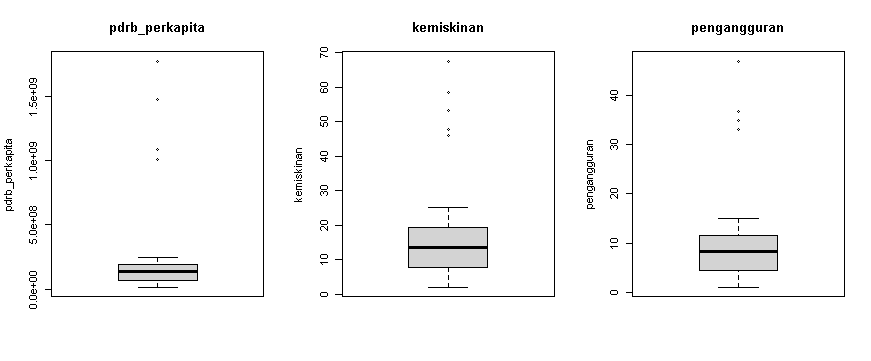
\includegraphics[width=15cm]{../gambar/boxplot_outlier.png}
\end{center}

\begin{center}
  \textbf{Tabel 3.4 Nilai-Nilai \textit{Outliers} yang Terdeteksi}
  
  \begin{tabular}{|c|c|c|}
  \hline
  \textbf{pdrb\_perkapita} & \textbf{kemiskinan} & \textbf{pengangguran} \\
  \hline
  1.012.449.971 & 45,95 & 33,19 \\
  \hline
  1.087.231.959 & 47,69 & 34,90 \\
  \hline
  1.472.419.961 & 53,50 & 36,68 \\
  \hline
  1.474.832.345 & 58,41 & 36,74 \\
  \hline
  1.774.545.027 & 67,53 & 47,04 \\
  \hline
  \end{tabular}
\end{center}

Dalam analisis ini, metode deteksi \textit{outliers} yang kami gunakan
adalah \textbf{IQR}. Metode ini mengidentifikasi \textit{outliers}
dengan menghitung rentang antara kuartil pertama (Q1) dan kuartil ketiga
(Q3). Nilai yang berada diluar rentang {[}Q1 - 1.5 x IQR, Q3 + 1.5 x
IQR{]} dianggap sebagai \textit{outliers}.

Nilai \textit{outliers} juga memiliki dampak besar terhadap analisis
statistik, salah satu contohnya adalah, \textit{outliers} dapat menarik
ukuran pemusatan data ke arah nilai ekstrem. Berikut tabel dampak nilai
\textit{outliers} yang sudah di analisis.

\begin{center}
  \textbf{Tabel 3.5 Dampak \textit{Outliers} terhadap Nilai Rata-Rata}
  
  \begin{tabular}{|c|c|c|c|}
  \hline
  \textbf{Variabel} & \textbf{Mean Sebelum Penghapusan} & \textbf{Mean Setelah Penghapusan} & \textbf{Selisih} \\
  \hline
  pdrb\_perkapita & 135.650.462 & 133.163.326 & 2.487.136 \\
  \hline
  kemiskinan & 13.72 & 13.64 & 0.08 \\
  \hline
  pengangguran & 8.05 & 7.99 & 0.06 \\
  \hline
  \end{tabular}
\end{center}

Variabel \textit{pdrb\_perkapita} mengalami perubahan rata-rata terbesar
setelah \textit{outlier} dihapus, yaitu sebesar 2.487.136. Ini
menunjukkan bahwa keberadaan beberapa daerah dengan nilai
\textit{pdrb\_perkapita} yang sangat tinggi memberikan pengaruh yang
cukup besar terhadap nilai rata-rata keseluruhan. Sementara itu,
variabel kemiskinan dan pengangguran hanya mengalami perubahan rata-rata
yang relatif kecil, sehingga pengaruh \textit{outlier} terhadap kedua
variabel tersebut tidak sebesar pada variabel \textit{pdrb\_perkapita}.

\subsection{\texorpdfstring{\normalsize 3.4 \hspace {0,5cm} Visualisasi
Data}{3.4  Visualisasi Data}}\label{visualisasi-data}

Visualisasi data merupakan salah satu teknik analisis yang digunakan
untuk menyajikan informasi dalam bentuk grafik sehingga pola, tren,
serta karakteristik data dapat dipahami dengan lebih mudah. Pada
penelitian ini, visualisasi dilakukan menggunakan library \emph{ggplot2}
pada bahasa pemrograman R untuk membantu proses interpretasi data
pembangunan wilayah di Indonesia.

Beberapa jenis visualisasi yang digunakan meliputi histogram, boxplot,
dan scatter plot. Histogram digunakan untuk melihat distribusi data pada
variabel \emph{ipm} dan \emph{kemiskinan}, boxplot digunakan untuk
mengidentifikasi keberadaan \emph{outlier} pada variabel
\emph{pdrb\_perkapita}, sedangkan scatter plot digunakan untuk mengamati
hubungan antar variabel pembangunan wilayah.

\begin{center}
\textbf{Gambar 3.2 Histogram Nilai IPM}

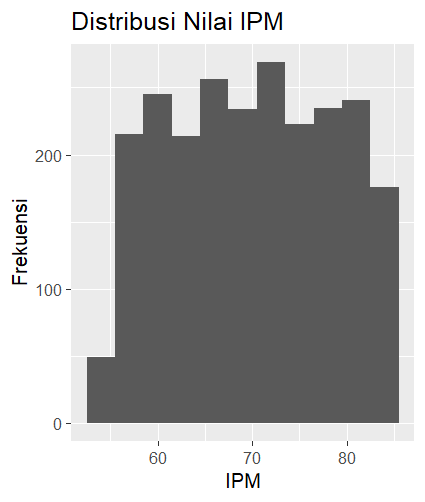
\includegraphics[width=12cm]{../gambar/histogramIPM.png}
\end{center}

Berdasarkan histogram nilai IPM, sebagian besar data terkonsentrasi pada
rentang nilai menengah hingga tinggi. Hal ini menunjukkan bahwa
mayoritas kabupaten/kota di Indonesia memiliki tingkat pembangunan
manusia yang relatif baik. Distribusi data juga terlihat cukup terpusat
dengan penyebaran yang tidak terlalu ekstrem.

\begin{center}
\textbf{Gambar 3.3 Histogram Tingkat Kemiskinan}

\includegraphics[width=12cm]{../gambar/histogram_kemiskinan.png}
\end{center}

Histogram tingkat kemiskinan menunjukkan bahwa sebagian besar wilayah
memiliki persentase kemiskinan pada kategori rendah hingga sedang. Namun
demikian, terdapat beberapa wilayah dengan tingkat kemiskinan yang
relatif tinggi sehingga menyebabkan distribusi data cenderung memanjang
pada bagian kanan.

\begin{center}
\textbf{Gambar 3.4 Boxplot PDRB Per Kapita}

\includegraphics[width=12cm]{../gambar/boxplot_pdrb.png}
\end{center}

Boxplot variabel \emph{pdrb\_perkapita} menunjukkan adanya beberapa
nilai ekstrem yang berada di luar batas whisker. Hasil ini sejalan
dengan analisis \emph{outlier} sebelumnya yang menunjukkan bahwa
terdapat sejumlah wilayah dengan nilai PDRB per kapita yang jauh lebih
tinggi dibandingkan mayoritas wilayah lainnya.

\begin{center}
\textbf{Gambar 3.5 Scatter Plot Kemiskinan dan IPM}


\includegraphics[width=12cm]{../gambar/scatter_kemiskinan_ipm.png}
\end{center}

Scatter plot antara tingkat kemiskinan dan IPM menunjukkan adanya
kecenderungan hubungan negatif. Secara umum, wilayah dengan tingkat
kemiskinan yang lebih tinggi cenderung memiliki nilai IPM yang lebih
rendah. Akan tetapi, pola hubungan yang terbentuk tidak terlalu kuat
karena penyebaran titik data masih cukup luas.

\begin{center}
\textbf{Gambar 3.6 Scatter Plot Akses Internet dan Rata-rata Lama Sekolah}


\includegraphics[width=12cm]{../gambar/scatter_internet_sekolah.png}
\end{center}

Hubungan antara akses internet dan rata-rata lama sekolah menunjukkan
kecenderungan hubungan positif. Wilayah dengan akses internet yang lebih
tinggi umumnya memiliki rata-rata lama sekolah yang lebih baik. Meskipun
demikian, penyebaran titik yang cukup luas menunjukkan bahwa terdapat
faktor lain yang turut memengaruhi tingkat pendidikan masyarakat.

Secara keseluruhan, visualisasi data memberikan gambaran yang lebih
jelas mengenai karakteristik pembangunan wilayah di Indonesia. Hasil
visualisasi juga mendukung analisis sebelumnya terkait keberadaan
\emph{outlier} serta adanya variasi kondisi pembangunan antarwilayah.

\subsection{\texorpdfstring{\normalsize 3.5 \hspace {0,5cm} Distribusi
Data}{3.5  Distribusi Data}}\label{distribusi-data}

Analisis distribusi data dilakukan untuk mengetahui karakteristik
sebaran data serta menilai apakah data mengikuti distribusi normal atau
tidak. Pada penelitian ini digunakan uji normalitas Shapiro-Wilk
terhadap beberapa variabel, yaitu \textit{ipm}, \textit{kemiskinan}, dan
\textit{akses_internet}. Selain itu, distribusi data juga diamati
menggunakan QQ Plot untuk membandingkan distribusi data aktual dengan
distribusi normal teoritis.

\begin{center}
\textbf{Tabel 3.6 Hasil Uji Normalitas Shapiro-Wilk}

\begin{tabular}{|c|c|c|}
\hline
\textbf{Variabel} & \textbf{P-Value} & \textbf{Kesimpulan} \
\hline
IPM & ISI_HASIL_R & ISI_HASIL_R \
\hline
Kemiskinan & ISI_HASIL_R & ISI_HASIL_R \
\hline
Akses Internet & ISI_HASIL_R & ISI_HASIL_R \
\hline
\end{tabular}
\end{center}

Akses Internet \& ISI\_HASIL\_R \& ISI\_HASIL\_R\\
\hline \textbackslash end\{tabular\} \textbackslash end\{center\}

Uji normalitas Shapiro-Wilk dilakukan dengan tingkat signifikansi
sebesar 5\% (\(\alpha = 0,05\)). Apabila nilai \textit{p-value} lebih
besar dari 0,05 maka data dianggap berdistribusi normal. Sebaliknya,
apabila nilai \textit{p-value} lebih kecil dari 0,05 maka data
dinyatakan tidak berdistribusi normal.

\begin{center}
\textbf{Gambar 3.7 QQ Plot Variabel IPM}

\includegraphics[width=12cm]{../gambar/qqplot_ipm.png}
\end{center}

\begin{center}
\textbf{Gambar 3.8 QQ Plot Variabel Kemiskinan}

\includegraphics[width=12cm]{../gambar/qqplot_kemiskinan.png}
\end{center}

\begin{center}
\textbf{Gambar 3.9 QQ Plot Variabel Akses Internet}

\includegraphics[width=12cm]{../gambar/qqplot_akses_internet.png}
\end{center}

Berdasarkan hasil visualisasi QQ Plot, sebagian besar titik data berada
di sekitar garis diagonal. Hal ini menunjukkan bahwa distribusi data
masih memiliki kemiripan dengan distribusi normal. Akan tetapi, pada
bagian ekor distribusi terdapat beberapa titik yang menyimpang dari
garis referensi sehingga menunjukkan adanya deviasi terhadap distribusi
normal sempurna.

Penyimpangan tersebut kemungkinan dipengaruhi oleh variasi kondisi
pembangunan antarwilayah serta keberadaan nilai ekstrem yang telah
teridentifikasi pada analisis \textit{outlier}. Faktor tersebut
menyebabkan distribusi data menjadi tidak sepenuhnya simetris.

Selain analisis distribusi, dilakukan pula analisis probabilitas untuk
memperoleh gambaran peluang terjadinya suatu kondisi pada data
pembangunan wilayah. Analisis probabilitas dilakukan menggunakan peluang
empiris berdasarkan data aktual serta fungsi distribusi normal pada
variabel IPM.

Hasil perhitungan menunjukkan peluang suatu wilayah memiliki tingkat
kemiskinan di atas rata-rata sebesar \textbf{ISI_HASIL_R}. Sementara
itu, peluang suatu wilayah memiliki nilai IPM lebih dari 75 adalah
sebesar \textbf{ISI_HASIL_R}. Berdasarkan pendekatan distribusi normal,
peluang nilai IPM kurang dari 75 diperoleh sebesar \textbf{ISI_HASIL_R}.

Selain itu, hasil perhitungan persentil ke-95 menunjukkan bahwa nilai
IPM sebesar \textbf{ISI_HASIL_R} dapat dijadikan batas atas yang hanya
dicapai oleh sekitar 5\% wilayah dengan tingkat pembangunan manusia
tertinggi.

Secara umum, hasil uji normalitas, QQ Plot, dan analisis probabilitas
menunjukkan bahwa karakteristik distribusi data berbeda untuk setiap
variabel. Oleh karena itu, interpretasi hasil analisis statistik perlu
mempertimbangkan asumsi distribusi data yang digunakan agar kesimpulan
yang diperoleh lebih akurat.

\subsection{\texorpdfstring{\normalsize 3.6 \hspace {0,5cm}
Korelasi}{3.6  Korelasi}}\label{korelasi}

Analisis korelasi merupakan metode statistik yang digunakan untuk
mengetahui hubungan antar variabel dalam suatu dataset. Pada penelitian
ini, analisis korelasi dilakukan menggunakan metode \textit{Pearson}
untuk mengukur kekuatan serta arah hubungan linear antar variabel
pembangunan wilayah.

Variabel yang dianalisis meliputi \textit{pdrb\_perkapita},
\textit{kemiskinan}, \textit{pengangguran}, \textit{ipm},
\textit{harapan\_hidup}, \textit{rata\_lama\_sekolah}, dan
\textit{akses\_internet}. Hasil analisis korelasi ditampilkan dalam
bentuk ringkasan berikut.

\begin{center}
  \textbf{Tabel 3.6 Hasil Analisis Korelasi}
  
  \begin{tabular}{|c|c|c|c|}
  \hline
  \textbf{Variabel 1} & \textbf{Variabel 2} & \textbf{Nilai Korelasi} & \textbf{Keterangan} \\
  \hline
  pdrb\_perkapita & kemiskinan & -0,0048 & Sangat lemah (negatif) \\
  \hline
  pengangguran & pdrb\_perkapita & -0,0323 & Sangat lemah (negatif) \\
  \hline
  ipm & pdrb\_perkapita & 0,0111 & Sangat lemah (positif) \\
  \hline
  harapan\_hidup & pdrb\_perkapita & 0,0125 & Sangat lemah (positif) \\
  \hline
  akses\_internet & kemiskinan & -0,0309 & Sangat lemah (negatif) \\
  \hline
  akses\_internet & ipm & 0,0020 & Sangat lemah (positif) \\
  \hline
  \end{tabular}
\end{center}

Berdasarkan hasil analisis, seluruh nilai korelasi berada sangat dekat
dengan nol, yaitu dalam rentang sekitar -0,03 hingga 0,01. Hal ini
menunjukkan bahwa hubungan linear antar variabel dalam dataset
pembangunan wilayah sangat lemah.

Tidak adanya korelasi yang kuat mengindikasikan bahwa variabel-variabel
tersebut tidak memiliki hubungan linear yang signifikan dan kemungkinan
dipengaruhi oleh faktor lain di luar model yang digunakan.

\subsection{\texorpdfstring{\normalsize 3.7 \hspace {0,5cm}
Interpretasi}{3.7  Interpretasi}}\label{interpretasi}

\setcounter{page}{3}

\newpage

\begin{center}
  {
    \bfseries
    
    \vfill
    
    \Large
    
    BAB IV
    
    KESIMPULAN
  }
\end{center}

\subsection{\texorpdfstring{\normalsize 4.1 \hspace {0,5cm} Kesimpulan
Utama}{4.1  Kesimpulan Utama}}\label{kesimpulan-utama}

Berdasarkan hasil analisis data pembangunan wilayah menggunakan bahasa
pemrograman R, dapat disimpulkan bahwa dataset memiliki kualitas yang
baik dengan tingkat \emph{missing value} yang sangat rendah, yaitu
sekitar 0,45\% dari keseluruhan data. Penanganan \emph{missing value}
dilakukan dengan metode penghapusan karena proporsinya relatif kecil dan
tidak memengaruhi representativitas data secara signifikan.

Analisis statistika deskriptif menunjukkan bahwa variabel ekonomi
memiliki tingkat variasi yang lebih tinggi dibandingkan variabel
pembangunan manusia. Selain itu, analisis \emph{outlier} menunjukkan
adanya beberapa data ekstrem pada variabel PDRB per kapita, kemiskinan,
dan pengangguran.

Hasil analisis korelasi menunjukkan bahwa hubungan antar indikator
pembangunan dalam dataset cenderung lemah dan tidak signifikan secara
statistik. Dengan demikian, pembangunan wilayah merupakan fenomena yang
kompleks dan dipengaruhi oleh berbagai faktor yang saling berkaitan.

\subsection{\texorpdfstring{\normalsize 4.2 \hspace {0,5cm}
Insight}{4.2  Insight}}\label{insight}

\begin{enumerate}
\def\labelenumi{\arabic{enumi}.}
\tightlist
\item
  Ketimpangan ekonomi antar wilayah masih terlihat dari adanya outlier
  pada variabel PDRB per kapita.
\item
  Variabel pembangunan manusia seperti IPM, harapan hidup, dan rata-rata
  lama sekolah memiliki distribusi yang relatif stabil.
\item
  Hubungan antar indikator pembangunan pada dataset tidak menunjukkan
  pola linear yang kuat.
\item
  Analisis pembangunan wilayah memerlukan pendekatan multivariat karena
  satu indikator tidak cukup menjelaskan kondisi pembangunan secara
  keseluruhan.
\end{enumerate}

\subsection{\texorpdfstring{\normalsize 4.3 \hspace {0,5cm}
Saran}{4.3  Saran}}\label{saran}

\begin{enumerate}
\def\labelenumi{\arabic{enumi}.}
\tightlist
\item
  Menambahkan variabel lain seperti investasi daerah, tingkat
  urbanisasi, dan pengeluaran pemerintah agar analisis lebih
  komprehensif.
\item
  Melakukan analisis regresi atau machine learning untuk
  mengidentifikasi faktor yang paling berpengaruh terhadap pembangunan
  wilayah.
\item
  Melakukan visualisasi yang lebih mendalam menggunakan histogram,
  scatter plot, dan heatmap korelasi.
\item
  Memperbarui dataset secara berkala agar hasil analisis dapat
  mencerminkan kondisi pembangunan yang lebih aktual.
\end{enumerate}

\setcounter{page}{4}

\newpage

\begin{center}
  {
    \bfseries
    
    \vfill
    
    \Large
    
    LAMPIRAN
  }
\end{center}

\subsection{\texorpdfstring{\normalsize 5.1 \hspace {0,5cm} Script
R}{5.1  Script R}}\label{script-r}

\begin{Shaded}
\begin{Highlighting}[]
\CommentTok{\# ======================}
\CommentTok{\# 1.3.1 Memahami Dataset}
\CommentTok{\# ======================}
\NormalTok{data\_pembangunan }\OtherTok{\textless{}{-}} \FunctionTok{read.csv}\NormalTok{(}\StringTok{"../dataset/pembangunan\_wilayah\_missing\_outlier.csv"}\NormalTok{)}
\NormalTok{(}\StringTok{"{-}{-}{-} STRUKTUR DATA {-}{-}{-}"}\NormalTok{)}
\FunctionTok{str}\NormalTok{(data\_pembangunan)}

\NormalTok{(}\StringTok{"{-}{-}{-} 6 BARIS PERTAMA DATASET {-}{-}{-}"}\NormalTok{)}
\FunctionTok{head}\NormalTok{(data\_pembangunan)}

\NormalTok{(}\StringTok{"{-}{-}{-} SUMMARY {-}{-}{-}"}\NormalTok{)}
\FunctionTok{summary}\NormalTok{(data\_pembangunan)}

\NormalTok{dimensi }\OtherTok{\textless{}{-}} \FunctionTok{dim}\NormalTok{(data\_pembangunan)}
\FunctionTok{cat}\NormalTok{(}\StringTok{"Jumlah Observasi (Baris) :"}\NormalTok{, dimensi[}\DecValTok{1}\NormalTok{])}
\FunctionTok{cat}\NormalTok{(}\StringTok{"Jumlah Variabel (Kolom)  :"}\NormalTok{, dimensi[}\DecValTok{2}\NormalTok{])}

\CommentTok{\# ===========================}
\CommentTok{\# 1.3.2 Statistika Deskriptif}
\CommentTok{\# ===========================}
\NormalTok{(}\StringTok{"{-}{-}{-} Mengambil variabel numerik {-}{-}{-}"}\NormalTok{)}
\NormalTok{data\_numerik }\OtherTok{\textless{}{-}}\NormalTok{ data\_pembangunan[}\FunctionTok{sapply}\NormalTok{(data\_pembangunan, is.numeric)]}

\NormalTok{(}\StringTok{"{-}{-}{-} Ringkasan statistik deskriptif {-}{-}{-}"}\NormalTok{)}
\FunctionTok{summary}\NormalTok{(data\_numerik)}

\NormalTok{(}\StringTok{"{-}{-}{-} Mean {-}{-}{-}"}\NormalTok{)}
\FunctionTok{sapply}\NormalTok{(data\_numerik, mean, }\AttributeTok{na.rm =} \ConstantTok{TRUE}\NormalTok{)}

\NormalTok{(}\StringTok{"{-}{-}{-} Median {-}{-}{-}"}\NormalTok{)}
\FunctionTok{sapply}\NormalTok{(data\_numerik, median, }\AttributeTok{na.rm =} \ConstantTok{TRUE}\NormalTok{)}

\NormalTok{(}\StringTok{"{-}{-}{-} Nilai minimum {-}{-}{-}"}\NormalTok{)}
\FunctionTok{sapply}\NormalTok{(data\_numerik, min, }\AttributeTok{na.rm =} \ConstantTok{TRUE}\NormalTok{)}

\NormalTok{(}\StringTok{"{-}{-}{-} Nilai maksimum {-}{-}{-}"}\NormalTok{)}
\FunctionTok{sapply}\NormalTok{(data\_numerik, max, }\AttributeTok{na.rm =} \ConstantTok{TRUE}\NormalTok{)}

\NormalTok{(}\StringTok{"{-}{-}{-} Standar deviasi {-}{-}{-}"}\NormalTok{)}
\FunctionTok{sapply}\NormalTok{(data\_numerik, sd, }\AttributeTok{na.rm =} \ConstantTok{TRUE}\NormalTok{)}

\NormalTok{(}\StringTok{"{-}{-}{-} Varians {-}{-}{-}"}\NormalTok{)}
\FunctionTok{sapply}\NormalTok{(data\_numerik, var, }\AttributeTok{na.rm =} \ConstantTok{TRUE}\NormalTok{)}

\NormalTok{(}\StringTok{"{-}{-}{-} Kuartil {-}{-}{-}"}\NormalTok{)}
\FunctionTok{sapply}\NormalTok{(data\_numerik, quantile, }\AttributeTok{na.rm =} \ConstantTok{TRUE}\NormalTok{)}

\CommentTok{\# ============================}
\CommentTok{\# 1.3.3 Analisis Missing Value}
\CommentTok{\# ============================}
\NormalTok{(}\StringTok{"{-}{-}{-} Memeriksa jumlah missing value di tiap variabel {-}{-}{-}"}\NormalTok{)}
\NormalTok{missing\_value }\OtherTok{\textless{}{-}} \FunctionTok{colSums}\NormalTok{(}\FunctionTok{is.na}\NormalTok{(data\_pembangunan))}

\NormalTok{(}\StringTok{"{-}{-}{-} Merepresentasikan jumlah missing value tiap variabel ke dalam persentase {-}{-}{-}"}\NormalTok{)}
\NormalTok{percentage\_missing\_value }\OtherTok{\textless{}{-}}\NormalTok{ missing\_value }\SpecialCharTok{/} \FunctionTok{nrow}\NormalTok{(data\_pembangunan) }\SpecialCharTok{*} \DecValTok{100}

\NormalTok{(}\StringTok{"{-}{-}{-} Menghitung rata{-}rata persentase missing value dataframe (secara keseluruhan) {-}{-}{-}"}\NormalTok{)}
\NormalTok{percentage\_missing\_value\_df }\OtherTok{\textless{}{-}} \FunctionTok{mean}\NormalTok{(}\FunctionTok{is.na}\NormalTok{(data\_pembangunan)) }\SpecialCharTok{*} \DecValTok{100}

\NormalTok{(}\StringTok{"{-}{-}{-} Melihat hasil perhitungan persentase {-}{-}{-}"}\NormalTok{)}
\FunctionTok{print}\NormalTok{(percentage\_missing\_value\_df)}

\NormalTok{(}\StringTok{"{-}{-}{-} Karena persentase 0.4\% \textless{} 30\%, maka metode yang diambil adalah metode penghapusan {-}{-}{-}"}\NormalTok{)}
\NormalTok{data\_pembangunan }\OtherTok{\textless{}{-}} \FunctionTok{na.omit}\NormalTok{(data\_pembangunan)}

\NormalTok{(}\StringTok{"{-}{-}{-} Memeriksa kembali apakah jumlah baris dataset sudah diperbarui setelah penghapusan {-}{-}{-}"}\NormalTok{)}
\FunctionTok{print}\NormalTok{(}\FunctionTok{nrow}\NormalTok{(data\_pembangunan))}

\CommentTok{\# ======================}
\CommentTok{\# 1.3.4 Analisis Outlier}
\CommentTok{\# ======================}
\NormalTok{(}\StringTok{"{-}{-}{-} Mengambil kolom variabel yang bertipe data numerik {-}{-}{-}"}\NormalTok{)}
\NormalTok{numeric\_columns\_name }\OtherTok{\textless{}{-}} \FunctionTok{names}\NormalTok{(data\_pembangunan)[}\FunctionTok{sapply}\NormalTok{(data\_pembangunan, is.numeric)]}

\NormalTok{outlier\_columns }\OtherTok{\textless{}{-}} \FunctionTok{c}\NormalTok{()}

\NormalTok{(}\StringTok{"{-}{-}{-} Menghitung IQR tiap kolom numerik {-}{-}{-}"}\NormalTok{)}
\ControlFlowTok{for}\NormalTok{(column\_name }\ControlFlowTok{in}\NormalTok{ numeric\_columns\_name) \{}
\NormalTok{  (}\StringTok{"{-}{-}{-} Mengambil kolom variabel yang bertipe data numerik {-}{-}{-}"}\NormalTok{)}
\NormalTok{  numeric\_columns\_name }\OtherTok{\textless{}{-}} \FunctionTok{names}\NormalTok{(data\_pembangunan)[}\FunctionTok{sapply}\NormalTok{(data\_pembangunan, is.numeric)]}
  
\NormalTok{  outlier\_columns }\OtherTok{\textless{}{-}} \FunctionTok{c}\NormalTok{()}
  
\NormalTok{  (}\StringTok{"{-}{-}{-} Menghitung IQR tiap kolom numerik {-}{-}{-}"}\NormalTok{)}
  \ControlFlowTok{for}\NormalTok{(column\_name }\ControlFlowTok{in}\NormalTok{ numeric\_columns\_name) \{}
  
\NormalTok{    Q1 }\OtherTok{\textless{}{-}} \FunctionTok{quantile}\NormalTok{(data\_pembangunan[[column\_name]], }\FloatTok{0.25}\NormalTok{, }\AttributeTok{na.rm =} \ConstantTok{TRUE}\NormalTok{)}
\NormalTok{    Q3 }\OtherTok{\textless{}{-}} \FunctionTok{quantile}\NormalTok{(data\_pembangunan[[column\_name]], }\FloatTok{0.75}\NormalTok{, }\AttributeTok{na.rm =} \ConstantTok{TRUE}\NormalTok{)}
  
\NormalTok{    IQR }\OtherTok{\textless{}{-}}\NormalTok{ Q3 }\SpecialCharTok{{-}}\NormalTok{ Q1}
  
\NormalTok{    lower\_bound }\OtherTok{\textless{}{-}}\NormalTok{ Q1 }\SpecialCharTok{{-}} \FloatTok{1.5} \SpecialCharTok{*}\NormalTok{ IQR}
\NormalTok{    upper\_bound }\OtherTok{\textless{}{-}}\NormalTok{ Q3 }\SpecialCharTok{+} \FloatTok{1.5} \SpecialCharTok{*}\NormalTok{ IQR}
  
\NormalTok{    outlier\_values }\OtherTok{\textless{}{-}}\NormalTok{ data\_pembangunan[[column\_name]][}
\NormalTok{      data\_pembangunan[[column\_name]] }\SpecialCharTok{\textless{}}\NormalTok{ lower\_bound }\SpecialCharTok{|}
\NormalTok{      data\_pembangunan[[column\_name]] }\SpecialCharTok{\textgreater{}}\NormalTok{ upper\_bound}
\NormalTok{    ]}
  
\NormalTok{    total\_outlier }\OtherTok{\textless{}{-}} \FunctionTok{length}\NormalTok{(outlier\_values)}
  
    \FunctionTok{cat}\NormalTok{(}\StringTok{"}\SpecialCharTok{\textbackslash{}n}\StringTok{====================================}\SpecialCharTok{\textbackslash{}n}\StringTok{"}\NormalTok{)}
    \FunctionTok{cat}\NormalTok{(}\StringTok{"Variabel :"}\NormalTok{, column\_name, }\StringTok{"}\SpecialCharTok{\textbackslash{}n}\StringTok{"}\NormalTok{)}
    \FunctionTok{cat}\NormalTok{(}\StringTok{"Jumlah Outlier :"}\NormalTok{, total\_outlier, }\StringTok{"}\SpecialCharTok{\textbackslash{}n}\StringTok{"}\NormalTok{)}
  
    \ControlFlowTok{if}\NormalTok{(total\_outlier }\SpecialCharTok{\textgreater{}} \DecValTok{0}\NormalTok{) \{}
  
\NormalTok{      outlier\_columns }\OtherTok{\textless{}{-}} \FunctionTok{c}\NormalTok{(outlier\_columns, column\_name)}
  
      \FunctionTok{cat}\NormalTok{(}\StringTok{"}\SpecialCharTok{\textbackslash{}n}\StringTok{Nilai Outlier:}\SpecialCharTok{\textbackslash{}n}\StringTok{"}\NormalTok{)}
      \FunctionTok{print}\NormalTok{(outlier\_values)}
  
\NormalTok{      mean\_sebelum }\OtherTok{\textless{}{-}} \FunctionTok{mean}\NormalTok{(}
\NormalTok{        data\_pembangunan[[column\_name]],}
        \AttributeTok{na.rm =} \ConstantTok{TRUE}
\NormalTok{      )}
  
\NormalTok{      data\_tanpa\_outlier }\OtherTok{\textless{}{-}}\NormalTok{ data\_pembangunan[[column\_name]][}
\NormalTok{        data\_pembangunan[[column\_name]] }\SpecialCharTok{\textgreater{}=}\NormalTok{ lower\_bound }\SpecialCharTok{\&}
\NormalTok{        data\_pembangunan[[column\_name]] }\SpecialCharTok{\textless{}=}\NormalTok{ upper\_bound}
\NormalTok{      ]}
  
\NormalTok{      mean\_setelah }\OtherTok{\textless{}{-}} \FunctionTok{mean}\NormalTok{(}
\NormalTok{        data\_tanpa\_outlier,}
        \AttributeTok{na.rm =} \ConstantTok{TRUE}
\NormalTok{      )}
  
      \FunctionTok{cat}\NormalTok{(}\StringTok{"}\SpecialCharTok{\textbackslash{}n}\StringTok{Rata{-}rata Outlier :"}\NormalTok{, }\FunctionTok{mean}\NormalTok{(outlier\_values), }\StringTok{"}\SpecialCharTok{\textbackslash{}n}\StringTok{"}\NormalTok{)}
      \FunctionTok{cat}\NormalTok{(}\StringTok{"Mean Sebelum :"}\NormalTok{, mean\_sebelum, }\StringTok{"}\SpecialCharTok{\textbackslash{}n}\StringTok{"}\NormalTok{)}
      \FunctionTok{cat}\NormalTok{(}\StringTok{"Mean Setelah :"}\NormalTok{, mean\_setelah, }\StringTok{"}\SpecialCharTok{\textbackslash{}n}\StringTok{"}\NormalTok{)}
      \FunctionTok{cat}\NormalTok{(}\StringTok{"Selisih Mean :"}\NormalTok{, }\FunctionTok{abs}\NormalTok{(mean\_sebelum }\SpecialCharTok{{-}}\NormalTok{ mean\_setelah), }\StringTok{"}\SpecialCharTok{\textbackslash{}n}\StringTok{"}\NormalTok{)}
\NormalTok{    \}}
\NormalTok{  \}}
\NormalTok{\}}

\NormalTok{(}\StringTok{"{-}{-}{-} Membuat boxplot hanya untuk variabel yang memiliki outlier {-}{-}{-}"}\NormalTok{)}
\FunctionTok{par}\NormalTok{(}\AttributeTok{mfrow =} \FunctionTok{c}\NormalTok{(}\DecValTok{1}\NormalTok{, }\FunctionTok{length}\NormalTok{(outlier\_columns)))}

\ControlFlowTok{for}\NormalTok{(col }\ControlFlowTok{in}\NormalTok{ outlier\_columns) \{}
  \FunctionTok{boxplot}\NormalTok{(}
\NormalTok{    data\_pembangunan[[col]],}
    \AttributeTok{main =}\NormalTok{ col,}
    \AttributeTok{ylab =}\NormalTok{ col}
\NormalTok{  )}
\NormalTok{\}}

\CommentTok{\# Bagian : 1.3.5 Visualisasi Data}
\CommentTok{\#          1.3.6 Analisis Probabilitas dan Distribusi Data}


\FunctionTok{library}\NormalTok{(ggplot2)}
\NormalTok{data }\OtherTok{\textless{}{-}} \FunctionTok{read.csv}\NormalTok{(}
  \StringTok{"data/pembangunan\_wilayah\_missing\_outlier.csv"}
\NormalTok{)}

\CommentTok{\#bersihin Missing Value}

\NormalTok{data\_clean }\OtherTok{\textless{}{-}} \FunctionTok{na.omit}\NormalTok{(data)}

\FunctionTok{cat}\NormalTok{(}\StringTok{"Jumlah data sebelum pembersihan :"}\NormalTok{, }\FunctionTok{nrow}\NormalTok{(data), }\StringTok{"}\SpecialCharTok{\textbackslash{}n}\StringTok{"}\NormalTok{)}
\FunctionTok{cat}\NormalTok{(}\StringTok{"Jumlah data setelah pembersihan :"}\NormalTok{, }\FunctionTok{nrow}\NormalTok{(data\_clean), }\StringTok{"}\SpecialCharTok{\textbackslash{}n}\StringTok{"}\NormalTok{)}

\CommentTok{\# =====================================================}
\CommentTok{\# 1.3.5 VISUALISASI DATA}
\CommentTok{\# =====================================================}

\CommentTok{\# Grafik 1 : Histogram IPM}

\FunctionTok{ggplot}\NormalTok{(data\_clean, }\FunctionTok{aes}\NormalTok{(}\AttributeTok{x =}\NormalTok{ ipm)) }\SpecialCharTok{+}
  \FunctionTok{geom\_histogram}\NormalTok{(}\AttributeTok{binwidth =} \DecValTok{3}\NormalTok{) }\SpecialCharTok{+}
  \FunctionTok{labs}\NormalTok{(}
    \AttributeTok{title =} \StringTok{"Distribusi Nilai IPM"}\NormalTok{,}
    \AttributeTok{x =} \StringTok{"IPM"}\NormalTok{,}
    \AttributeTok{y =} \StringTok{"Frekuensi"}
\NormalTok{  )}

\CommentTok{\# Grafik 2 : Histogram Kemiskinan}

\FunctionTok{ggplot}\NormalTok{(data\_clean, }\FunctionTok{aes}\NormalTok{(}\AttributeTok{x =}\NormalTok{ kemiskinan)) }\SpecialCharTok{+}
  \FunctionTok{geom\_histogram}\NormalTok{(}\AttributeTok{binwidth =} \DecValTok{2}\NormalTok{) }\SpecialCharTok{+}
  \FunctionTok{labs}\NormalTok{(}
    \AttributeTok{title =} \StringTok{"Distribusi Tingkat Kemiskinan"}\NormalTok{,}
    \AttributeTok{x =} \StringTok{"Kemiskinan (\%)"}\NormalTok{,}
    \AttributeTok{y =} \StringTok{"Frekuensi"}
\NormalTok{  )}

\CommentTok{\# Grafik 3 : Boxplot PDRB Per Kapita}

\FunctionTok{ggplot}\NormalTok{(data\_clean, }\FunctionTok{aes}\NormalTok{(}\AttributeTok{y =}\NormalTok{ pdrb\_perkapita)) }\SpecialCharTok{+}
  \FunctionTok{geom\_boxplot}\NormalTok{() }\SpecialCharTok{+}
  \FunctionTok{labs}\NormalTok{(}
    \AttributeTok{title =} \StringTok{"Boxplot PDRB Per Kapita"}\NormalTok{,}
    \AttributeTok{y =} \StringTok{"PDRB Per Kapita"}
\NormalTok{  )}

\CommentTok{\# Grafik 4 : Scatter Plot Kemiskinan vs IPM}

\FunctionTok{ggplot}\NormalTok{(data\_clean,}
       \FunctionTok{aes}\NormalTok{(}
         \AttributeTok{x =}\NormalTok{ kemiskinan,}
         \AttributeTok{y =}\NormalTok{ ipm}
\NormalTok{       )) }\SpecialCharTok{+}
  \FunctionTok{geom\_point}\NormalTok{() }\SpecialCharTok{+}
  \FunctionTok{labs}\NormalTok{(}
    \AttributeTok{title =} \StringTok{"Hubungan Kemiskinan dan IPM"}\NormalTok{,}
    \AttributeTok{x =} \StringTok{"Kemiskinan (\%)"}\NormalTok{,}
    \AttributeTok{y =} \StringTok{"IPM"}
\NormalTok{  )}

\CommentTok{\# Grafik 5 : Scatter Plot Akses Internet}
\CommentTok{\#             vs Rata Lama Sekolah}

\FunctionTok{ggplot}\NormalTok{(data\_clean,}
       \FunctionTok{aes}\NormalTok{(}
         \AttributeTok{x =}\NormalTok{ akses\_internet,}
         \AttributeTok{y =}\NormalTok{ rata\_lama\_sekolah}
\NormalTok{       )) }\SpecialCharTok{+}
  \FunctionTok{geom\_point}\NormalTok{() }\SpecialCharTok{+}
  \FunctionTok{labs}\NormalTok{(}
    \AttributeTok{title =} \StringTok{"Hubungan Akses Internet dan Rata Lama Sekolah"}\NormalTok{,}
    \AttributeTok{x =} \StringTok{"Akses Internet (\%)"}\NormalTok{,}
    \AttributeTok{y =} \StringTok{"Rata Lama Sekolah (Tahun)"}
\NormalTok{  )}

\CommentTok{\# =====================================================}
\CommentTok{\# 1.3.6 ANALISIS DISTRIBUSI DATA}
\CommentTok{\# =====================================================}

\CommentTok{\# Uji Normalitas Shapiro{-}Wilk}

\NormalTok{shapiro\_ipm }\OtherTok{\textless{}{-}} \FunctionTok{shapiro.test}\NormalTok{(data\_clean}\SpecialCharTok{$}\NormalTok{ipm)}
\NormalTok{shapiro\_kemiskinan }\OtherTok{\textless{}{-}} \FunctionTok{shapiro.test}\NormalTok{(data\_clean}\SpecialCharTok{$}\NormalTok{kemiskinan)}
\NormalTok{shapiro\_internet }\OtherTok{\textless{}{-}} \FunctionTok{shapiro.test}\NormalTok{(data\_clean}\SpecialCharTok{$}\NormalTok{akses\_internet)}

\FunctionTok{cat}\NormalTok{(}\StringTok{"}\SpecialCharTok{\textbackslash{}n}\StringTok{"}\NormalTok{)}
\FunctionTok{cat}\NormalTok{(}\StringTok{"===================================}\SpecialCharTok{\textbackslash{}n}\StringTok{"}\NormalTok{)}
\FunctionTok{cat}\NormalTok{(}\StringTok{"HASIL UJI NORMALITAS}\SpecialCharTok{\textbackslash{}n}\StringTok{"}\NormalTok{)}
\FunctionTok{cat}\NormalTok{(}\StringTok{"===================================}\SpecialCharTok{\textbackslash{}n}\StringTok{"}\NormalTok{)}

\FunctionTok{print}\NormalTok{(shapiro\_ipm)}
\FunctionTok{print}\NormalTok{(shapiro\_kemiskinan)}
\FunctionTok{print}\NormalTok{(shapiro\_internet)}

\CommentTok{\# QQ Plot IPM}

\FunctionTok{qqnorm}\NormalTok{(data\_clean}\SpecialCharTok{$}\NormalTok{ipm,}
       \AttributeTok{main =} \StringTok{"QQ Plot IPM"}\NormalTok{)}
\FunctionTok{qqline}\NormalTok{(data\_clean}\SpecialCharTok{$}\NormalTok{ipm)}

\CommentTok{\# QQ Plot Kemiskinan}

\FunctionTok{qqnorm}\NormalTok{(data\_clean}\SpecialCharTok{$}\NormalTok{kemiskinan,}
       \AttributeTok{main =} \StringTok{"QQ Plot Kemiskinan"}\NormalTok{)}
\FunctionTok{qqline}\NormalTok{(data\_clean}\SpecialCharTok{$}\NormalTok{kemiskinan)}

\CommentTok{\# =====================================================}
\CommentTok{\# ANALISIS PROBABILITAS}
\CommentTok{\# =====================================================}

\CommentTok{\# Probabilitas Kemiskinan}
\CommentTok{\# di atas rata{-}rata}

\NormalTok{mean\_kemiskinan }\OtherTok{\textless{}{-}} \FunctionTok{mean}\NormalTok{(data\_clean}\SpecialCharTok{$}\NormalTok{kemiskinan)}

\NormalTok{prob\_kemiskinan\_atas\_rata }\OtherTok{\textless{}{-}} \FunctionTok{mean}\NormalTok{(}
\NormalTok{  data\_clean}\SpecialCharTok{$}\NormalTok{kemiskinan }\SpecialCharTok{\textgreater{}}\NormalTok{ mean\_kemiskinan}
\NormalTok{)}

\FunctionTok{cat}\NormalTok{(}\StringTok{"}\SpecialCharTok{\textbackslash{}n}\StringTok{"}\NormalTok{)}
\FunctionTok{cat}\NormalTok{(}\StringTok{"===================================}\SpecialCharTok{\textbackslash{}n}\StringTok{"}\NormalTok{)}
\FunctionTok{cat}\NormalTok{(}\StringTok{"PROBABILITAS KEMISKINAN}\SpecialCharTok{\textbackslash{}n}\StringTok{"}\NormalTok{)}
\FunctionTok{cat}\NormalTok{(}\StringTok{"===================================}\SpecialCharTok{\textbackslash{}n}\StringTok{"}\NormalTok{)}

\FunctionTok{cat}\NormalTok{(}
  \StringTok{"Probabilitas wilayah memiliki kemiskinan di atas rata{-}rata = "}\NormalTok{,}
  \FunctionTok{round}\NormalTok{(prob\_kemiskinan\_atas\_rata,}\DecValTok{4}\NormalTok{),}
  \StringTok{"}\SpecialCharTok{\textbackslash{}n}\StringTok{"}
\NormalTok{)}

\CommentTok{\# Probabilitas IPM \textgreater{} 75}

\NormalTok{prob\_ipm\_tinggi }\OtherTok{\textless{}{-}} \FunctionTok{mean}\NormalTok{(}
\NormalTok{  data\_clean}\SpecialCharTok{$}\NormalTok{ipm }\SpecialCharTok{\textgreater{}} \DecValTok{75}
\NormalTok{)}

\FunctionTok{cat}\NormalTok{(}
  \StringTok{"Probabilitas wilayah memiliki IPM \textgreater{} 75 = "}\NormalTok{,}
  \FunctionTok{round}\NormalTok{(prob\_ipm\_tinggi,}\DecValTok{4}\NormalTok{),}
  \StringTok{"}\SpecialCharTok{\textbackslash{}n}\StringTok{"}
\NormalTok{)}

\CommentTok{\# Probabilitas Normal pakai pnorm()}
\CommentTok{\# P(IPM \textless{} 75)}

\NormalTok{prob\_normal\_ipm }\OtherTok{\textless{}{-}} \FunctionTok{pnorm}\NormalTok{(}
  \DecValTok{75}\NormalTok{,}
  \FunctionTok{mean}\NormalTok{(data\_clean}\SpecialCharTok{$}\NormalTok{ipm),}
  \FunctionTok{sd}\NormalTok{(data\_clean}\SpecialCharTok{$}\NormalTok{ipm)}
\NormalTok{)}

\FunctionTok{cat}\NormalTok{(}
  \StringTok{"Probabilitas IPM kurang dari 75 (Distribusi Normal) = "}\NormalTok{,}
  \FunctionTok{round}\NormalTok{(prob\_normal\_ipm,}\DecValTok{4}\NormalTok{),}
  \StringTok{"}\SpecialCharTok{\textbackslash{}n}\StringTok{"}
\NormalTok{)}

\CommentTok{\# Nilai IPM pada persentil ke{-}95}
\CommentTok{\# pakai qnorm()}

\NormalTok{ipm\_p95 }\OtherTok{\textless{}{-}} \FunctionTok{qnorm}\NormalTok{(}
  \FloatTok{0.95}\NormalTok{,}
  \FunctionTok{mean}\NormalTok{(data\_clean}\SpecialCharTok{$}\NormalTok{ipm),}
  \FunctionTok{sd}\NormalTok{(data\_clean}\SpecialCharTok{$}\NormalTok{ipm)}
\NormalTok{)}

\FunctionTok{cat}\NormalTok{(}
  \StringTok{"Nilai IPM pada persentil ke{-}95 = "}\NormalTok{,}
  \FunctionTok{round}\NormalTok{(ipm\_p95,}\DecValTok{2}\NormalTok{),}
  \StringTok{"}\SpecialCharTok{\textbackslash{}n}\StringTok{"}
\NormalTok{)}

\CommentTok{\# =====================================================}
\CommentTok{\# TABEL RINGKAS HASIL UJI NORMALITAS}
\CommentTok{\# =====================================================}

\NormalTok{hasil\_normalitas }\OtherTok{\textless{}{-}} \FunctionTok{data.frame}\NormalTok{(}
  \AttributeTok{Variabel =} \FunctionTok{c}\NormalTok{(}
    \StringTok{"IPM"}\NormalTok{,}
    \StringTok{"Kemiskinan"}\NormalTok{,}
    \StringTok{"Akses Internet"}
\NormalTok{  ),}
  \AttributeTok{P\_Value =} \FunctionTok{c}\NormalTok{(}
\NormalTok{    shapiro\_ipm}\SpecialCharTok{$}\NormalTok{p.value,}
\NormalTok{    shapiro\_kemiskinan}\SpecialCharTok{$}\NormalTok{p.value,}
\NormalTok{    shapiro\_internet}\SpecialCharTok{$}\NormalTok{p.value}
\NormalTok{  )}
\NormalTok{)}

\NormalTok{hasil\_normalitas}\SpecialCharTok{$}\NormalTok{Kesimpulan }\OtherTok{\textless{}{-}}
  \FunctionTok{ifelse}\NormalTok{(}
\NormalTok{    hasil\_normalitas}\SpecialCharTok{$}\NormalTok{P\_Value }\SpecialCharTok{\textgreater{}} \FloatTok{0.05}\NormalTok{,}
    \StringTok{"Berdistribusi Normal"}\NormalTok{,}
    \StringTok{"Tidak Berdistribusi Normal"}
\NormalTok{  )}

\FunctionTok{cat}\NormalTok{(}\StringTok{"}\SpecialCharTok{\textbackslash{}n}\StringTok{"}\NormalTok{)}
\FunctionTok{cat}\NormalTok{(}\StringTok{"===================================}\SpecialCharTok{\textbackslash{}n}\StringTok{"}\NormalTok{)}
\FunctionTok{cat}\NormalTok{(}\StringTok{"TABEL HASIL UJI NORMALITAS}\SpecialCharTok{\textbackslash{}n}\StringTok{"}\NormalTok{)}
\FunctionTok{cat}\NormalTok{(}\StringTok{"===================================}\SpecialCharTok{\textbackslash{}n}\StringTok{"}\NormalTok{)}

\FunctionTok{print}\NormalTok{(hasil\_normalitas)}


\CommentTok{\# ============================}
\CommentTok{\# 1.3.7 Analisis Korelasi}
\CommentTok{\# ============================}
\NormalTok{data\_bersih }\OtherTok{\textless{}{-}}\NormalTok{ data\_pembangunan[}\FunctionTok{complete.cases}\NormalTok{(data\_pembangunan), ]}
\NormalTok{kolom\_numerik\_korelasi }\OtherTok{\textless{}{-}} \FunctionTok{c}\NormalTok{(}\StringTok{"pdrb\_perkapita"}\NormalTok{, }\StringTok{"kemiskinan"}\NormalTok{, }\StringTok{"pengangguran"}\NormalTok{, }\StringTok{"ipm"}\NormalTok{, }
                            \StringTok{"harapan\_hidup"}\NormalTok{, }\StringTok{"rata\_lama\_sekolah"}\NormalTok{, }\StringTok{"akses\_internet"}\NormalTok{, }
                            \StringTok{"jalan\_baik"}\NormalTok{, }\StringTok{"air\_bersih"}\NormalTok{)}

\NormalTok{matriks\_numerik }\OtherTok{\textless{}{-}}\NormalTok{ data\_bersih[, kolom\_numerik\_korelasi]}

\FunctionTok{cat}\NormalTok{(}\StringTok{"{-}{-}{-} Menghitung korelasi antar variabel {-}{-}{-}"}\NormalTok{)}
\NormalTok{matriks\_korelasi }\OtherTok{\textless{}{-}} \FunctionTok{cor}\NormalTok{(matriks\_numerik, }\AttributeTok{method =} \StringTok{"pearson"}\NormalTok{)}
\FunctionTok{print}\NormalTok{(}\FunctionTok{round}\NormalTok{(matriks\_korelasi, }\DecValTok{3}\NormalTok{))}

\FunctionTok{cat}\NormalTok{(}\StringTok{"{-}{-}{-} UJI KORELASI: IPM vs KEMISKINAN {-}{-}{-}"}\NormalTok{)}
\NormalTok{uji\_ipm\_kemiskinan }\OtherTok{\textless{}{-}} \FunctionTok{cor.test}\NormalTok{(data\_bersih}\SpecialCharTok{$}\NormalTok{ipm, data\_bersih}\SpecialCharTok{$}\NormalTok{kemiskinan)}
\FunctionTok{print}\NormalTok{(uji\_ipm\_kemiskinan)}

\FunctionTok{cat}\NormalTok{(}\StringTok{"{-}{-}{-} UJI KORELASI: AKSES INTERNET vs RATA{-}LAMA SEKOLAH {-}{-}{-}"}\NormalTok{)}
\NormalTok{uji\_internet\_sekolah }\OtherTok{\textless{}{-}} \FunctionTok{cor.test}\NormalTok{(data\_bersih}\SpecialCharTok{$}\NormalTok{akses\_internet, data\_bersih}\SpecialCharTok{$}\NormalTok{rata\_lama\_sekolah)}
\FunctionTok{print}\NormalTok{(uji\_internet\_sekolah)}

\FunctionTok{cat}\NormalTok{(}\StringTok{"{-}{-}{-} UJI KORELASI: PDRB PERKAPITA vs IPM (KESEJAHTERAAN) {-}{-}{-}"}\NormalTok{)}
\NormalTok{uji\_pdrb\_ipm }\OtherTok{\textless{}{-}} \FunctionTok{cor.test}\NormalTok{(data\_bersih}\SpecialCharTok{$}\NormalTok{pdrb\_perkapita, data\_bersih}\SpecialCharTok{$}\NormalTok{ipm)}
\FunctionTok{print}\NormalTok{(uji\_pdrb\_ipm)}

\end{Highlighting}
\end{Shaded}

\subsection{\texorpdfstring{\normalsize 5.2 \hspace {0,5cm} Output
Tambahan}{5.2  Output Tambahan}}\label{output-tambahan}

\begin{verbatim}
##           wilayah          provinsi             tahun    pdrb_perkapita        kemiskinan 
##       "character"       "character"         "integer"         "numeric"         "numeric" 
##      pengangguran               ipm     harapan_hidup rata_lama_sekolah    akses_internet 
##         "numeric"         "numeric"         "numeric"         "numeric"         "numeric" 
##        jalan_baik        air_bersih      catatan_data 
##         "numeric"         "numeric"       "character"
\end{verbatim}

\begin{verbatim}
##            wilayah         provinsi tahun pdrb_perkapita kemiskinan pengangguran   ipm
## 1 Kabupaten/Kota_1       Jawa Barat  2022       38403994      19.69         4.73 80.16
## 2 Kabupaten/Kota_2       Jawa Timur  2022      165582092       9.68         4.43 55.05
## 3 Kabupaten/Kota_3 Kalimantan Timur  2020       26780948       4.13         2.99 78.70
## 4 Kabupaten/Kota_4      DKI Jakarta  2022      155034790      20.43         3.90 73.27
## 5 Kabupaten/Kota_5 Sulawesi Selatan  2023      198834591      14.39        12.15 72.90
## 6 Kabupaten/Kota_6       Jawa Timur  2020      145702606      17.14         3.38 65.11
##   harapan_hidup rata_lama_sekolah akses_internet jalan_baik air_bersih catatan_data
## 1         75.75              8.41          63.86      53.86      43.11       Normal
## 2         67.85              5.79          66.61      34.89      58.93       Normal
## 3         60.38             13.20          64.73      48.57      90.27       Normal
## 4         69.49             12.28          44.59      57.88      86.16       Normal
## 5         75.00              9.69          52.72      65.70      90.84       Normal
## 6         67.04              5.66          55.63      70.12      60.17       Normal
\end{verbatim}

\begin{verbatim}
##    wilayah            provinsi             tahun      pdrb_perkapita        kemiskinan   
##  Length:2500        Length:2500        Min.   :2020   Min.   :1.503e+07   Min.   : 2.01  
##  Class :character   Class :character   1st Qu.:2021   1st Qu.:6.962e+07   1st Qu.: 7.86  
##  Mode  :character   Mode  :character   Median :2022   Median :1.373e+08   Median :13.72  
##                                        Mean   :2022   Mean   :1.357e+08   Mean   :13.72  
##                                        3rd Qu.:2023   3rd Qu.:1.939e+08   3rd Qu.:19.39  
##                                        Max.   :2024   Max.   :1.775e+09   Max.   :67.53  
##                                                       NA's   :25          NA's   :24     
##   pengangguran         ipm        harapan_hidup   rata_lama_sekolah akses_internet 
##  Min.   : 1.010   Min.   :55.01   Min.   :60.01   Min.   : 5.020    Min.   : 0.01  
##  1st Qu.: 4.350   1st Qu.:62.52   1st Qu.:64.66   1st Qu.: 7.327    1st Qu.:38.91  
##  Median : 8.230   Median :69.89   Median :69.30   Median : 9.520    Median :58.09  
##  Mean   : 8.046   Mean   :69.90   Mean   :69.13   Mean   : 9.581    Mean   :58.79  
##  3rd Qu.:11.520   3rd Qu.:77.16   3rd Qu.:73.58   3rd Qu.:11.912    3rd Qu.:78.67  
##  Max.   :47.040   Max.   :84.99   Max.   :77.99   Max.   :14.000    Max.   :97.99  
##  NA's   :25       NA's   :25                                        NA's   :25     
##    jalan_baik      air_bersih    catatan_data      
##  Min.   :30.01   Min.   :40.03   Length:2500       
##  1st Qu.:47.40   1st Qu.:54.32   Class :character  
##  Median :65.02   Median :69.68   Mode  :character  
##  Mean   :65.26   Mean   :69.76                     
##  3rd Qu.:83.24   3rd Qu.:85.18                     
##  Max.   :99.95   Max.   :99.99                     
##  NA's   :25
\end{verbatim}

\begin{verbatim}
## Jumlah Observasi (Baris) : 2500
\end{verbatim}

\begin{verbatim}
## Jumlah Variabel (Kolom)  : 13
\end{verbatim}

\begin{verbatim}
##      tahun      pdrb_perkapita        kemiskinan     pengangguran         ipm       
##  Min.   :2020   Min.   :1.503e+07   Min.   : 2.01   Min.   : 1.010   Min.   :55.01  
##  1st Qu.:2021   1st Qu.:6.962e+07   1st Qu.: 7.86   1st Qu.: 4.350   1st Qu.:62.52  
##  Median :2022   Median :1.373e+08   Median :13.72   Median : 8.230   Median :69.89  
##  Mean   :2022   Mean   :1.357e+08   Mean   :13.72   Mean   : 8.046   Mean   :69.90  
##  3rd Qu.:2023   3rd Qu.:1.939e+08   3rd Qu.:19.39   3rd Qu.:11.520   3rd Qu.:77.16  
##  Max.   :2024   Max.   :1.775e+09   Max.   :67.53   Max.   :47.040   Max.   :84.99  
##                 NA's   :25          NA's   :24      NA's   :25       NA's   :25     
##  harapan_hidup   rata_lama_sekolah akses_internet    jalan_baik      air_bersih   
##  Min.   :60.01   Min.   : 5.020    Min.   : 0.01   Min.   :30.01   Min.   :40.03  
##  1st Qu.:64.66   1st Qu.: 7.327    1st Qu.:38.91   1st Qu.:47.40   1st Qu.:54.32  
##  Median :69.30   Median : 9.520    Median :58.09   Median :65.02   Median :69.68  
##  Mean   :69.13   Mean   : 9.581    Mean   :58.79   Mean   :65.26   Mean   :69.76  
##  3rd Qu.:73.58   3rd Qu.:11.912    3rd Qu.:78.67   3rd Qu.:83.24   3rd Qu.:85.18  
##  Max.   :77.99   Max.   :14.000    Max.   :97.99   Max.   :99.95   Max.   :99.99  
##                                    NA's   :25      NA's   :25
\end{verbatim}

\begin{verbatim}
##             tahun    pdrb_perkapita        kemiskinan      pengangguran               ipm 
##      2.021999e+03      1.356505e+08      1.372146e+01      8.045733e+00      6.989999e+01 
##     harapan_hidup rata_lama_sekolah    akses_internet        jalan_baik        air_bersih 
##      6.913015e+01      9.580684e+00      5.878903e+01      6.525808e+01      6.976153e+01
\end{verbatim}

\begin{verbatim}
##             tahun    pdrb_perkapita        kemiskinan      pengangguran               ipm 
##      2.022000e+03      1.373106e+08      1.372000e+01      8.230000e+00      6.989000e+01 
##     harapan_hidup rata_lama_sekolah    akses_internet        jalan_baik        air_bersih 
##      6.929500e+01      9.520000e+00      5.809000e+01      6.502000e+01      6.968000e+01
\end{verbatim}

\begin{verbatim}
##             tahun    pdrb_perkapita        kemiskinan      pengangguran               ipm 
##           2020.00       15031581.00              2.01              1.01             55.01 
##     harapan_hidup rata_lama_sekolah    akses_internet        jalan_baik        air_bersih 
##             60.01              5.02              0.01             30.01             40.03
\end{verbatim}

\begin{verbatim}
##             tahun    pdrb_perkapita        kemiskinan      pengangguran               ipm 
##      2.024000e+03      1.774545e+09      6.753000e+01      4.704000e+01      8.499000e+01 
##     harapan_hidup rata_lama_sekolah    akses_internet        jalan_baik        air_bersih 
##      7.799000e+01      1.400000e+01      9.799000e+01      9.995000e+01      9.999000e+01
\end{verbatim}

\begin{verbatim}
##             tahun    pdrb_perkapita        kemiskinan      pengangguran               ipm 
##      1.431789e+00      8.934127e+07      6.894704e+00      4.258576e+00      8.535062e+00 
##     harapan_hidup rata_lama_sekolah    akses_internet        jalan_baik        air_bersih 
##      5.171779e+00      2.627008e+00      2.282030e+01      2.036569e+01      1.749921e+01
\end{verbatim}

\begin{verbatim}
##             tahun    pdrb_perkapita        kemiskinan      pengangguran               ipm 
##      2.050019e+00      7.981863e+15      4.753694e+01      1.813547e+01      7.284728e+01 
##     harapan_hidup rata_lama_sekolah    akses_internet        jalan_baik        air_bersih 
##      2.674730e+01      6.901173e+00      5.207660e+02      4.147613e+02      3.062222e+02
\end{verbatim}

\begin{verbatim}
##      tahun pdrb_perkapita kemiskinan pengangguran   ipm harapan_hidup rata_lama_sekolah
## 0%    2020       15031581     2.0100         1.01 55.01       60.0100            5.0200
## 25%   2021       69622210     7.8600         4.35 62.52       64.6575            7.3275
## 50%   2022      137310624    13.7200         8.23 69.89       69.2950            9.5200
## 75%   2023      193899157    19.3925        11.52 77.16       73.5850           11.9125
## 100%  2024     1774545027    67.5300        47.04 84.99       77.9900           14.0000
##      akses_internet jalan_baik air_bersih
## 0%            0.010     30.010    40.0300
## 25%          38.915     47.395    54.3175
## 50%          58.090     65.020    69.6800
## 75%          78.670     83.240    85.1825
## 100%         97.990     99.950    99.9900
\end{verbatim}

\begin{verbatim}
## [1] 0.4584615
\end{verbatim}

\begin{verbatim}
## [1] 2357
\end{verbatim}

\begin{verbatim}
## [1] "--- Mengambil kolom variabel yang bertipe data numerik ---"
\end{verbatim}

\begin{verbatim}
## [1] "--- Menghitung IQR tiap kolom numerik ---"
\end{verbatim}

\begin{verbatim}
## 
## ====================================
## Variabel : tahun 
## Jumlah Outlier : 0 
## 
## ====================================
## Variabel : pdrb_perkapita 
## Jumlah Outlier : 5 
## 
## Nilai Outlier:
## [1] 1472419961 1474832345 1774545027 1087231959 1012449971
## 
## Rata-rata Outlier : 1364295853 
## Mean Sebelum : 135736399 
## Mean Setelah : 133124666 
## Selisih Mean : 2611734 
## 
## ====================================
## Variabel : kemiskinan 
## Jumlah Outlier : 5 
## 
## Nilai Outlier:
## [1] 45.95 53.30 67.53 47.69 58.41
## 
## Rata-rata Outlier : 54.576 
## Mean Sebelum : 13.68089 
## Mean Setelah : 13.59395 
## Selisih Mean : 0.08693689 
## 
## ====================================
## Variabel : pengangguran 
## Jumlah Outlier : 5 
## 
## Nilai Outlier:
## [1] 47.04 34.90 36.74 36.68 33.19
## 
## Rata-rata Outlier : 37.71 
## Mean Sebelum : 8.053271 
## Mean Setelah : 7.990225 
## Selisih Mean : 0.06304577 
## 
## ====================================
## Variabel : ipm 
## Jumlah Outlier : 0 
## 
## ====================================
## Variabel : harapan_hidup 
## Jumlah Outlier : 0 
## 
## ====================================
## Variabel : rata_lama_sekolah 
## Jumlah Outlier : 0 
## 
## ====================================
## Variabel : akses_internet 
## Jumlah Outlier : 0 
## 
## ====================================
## Variabel : jalan_baik 
## Jumlah Outlier : 0 
## 
## ====================================
## Variabel : air_bersih 
## Jumlah Outlier : 0 
## 
## ====================================
## Variabel : tahun 
## Jumlah Outlier : 0 
## 
## ====================================
## Variabel : pdrb_perkapita 
## Jumlah Outlier : 5 
## 
## Nilai Outlier:
## [1] 1472419961 1474832345 1774545027 1087231959 1012449971
## 
## Rata-rata Outlier : 1364295853 
## Mean Sebelum : 135736399 
## Mean Setelah : 133124666 
## Selisih Mean : 2611734 
## 
## ====================================
## Variabel : kemiskinan 
## Jumlah Outlier : 5 
## 
## Nilai Outlier:
## [1] 45.95 53.30 67.53 47.69 58.41
## 
## Rata-rata Outlier : 54.576 
## Mean Sebelum : 13.68089 
## Mean Setelah : 13.59395 
## Selisih Mean : 0.08693689 
## 
## ====================================
## Variabel : pengangguran 
## Jumlah Outlier : 5 
## 
## Nilai Outlier:
## [1] 47.04 34.90 36.74 36.68 33.19
## 
## Rata-rata Outlier : 37.71 
## Mean Sebelum : 8.053271 
## Mean Setelah : 7.990225 
## Selisih Mean : 0.06304577 
## 
## ====================================
## Variabel : ipm 
## Jumlah Outlier : 0 
## 
## ====================================
## Variabel : harapan_hidup 
## Jumlah Outlier : 0 
## 
## ====================================
## Variabel : rata_lama_sekolah 
## Jumlah Outlier : 0 
## 
## ====================================
## Variabel : akses_internet 
## Jumlah Outlier : 0 
## 
## ====================================
## Variabel : jalan_baik 
## Jumlah Outlier : 0 
## 
## ====================================
## Variabel : air_bersih 
## Jumlah Outlier : 0 
## 
## ====================================
## Variabel : tahun 
## Jumlah Outlier : 0 
## 
## ====================================
## Variabel : pdrb_perkapita 
## Jumlah Outlier : 5 
## 
## Nilai Outlier:
## [1] 1472419961 1474832345 1774545027 1087231959 1012449971
## 
## Rata-rata Outlier : 1364295853 
## Mean Sebelum : 135736399 
## Mean Setelah : 133124666 
## Selisih Mean : 2611734 
## 
## ====================================
## Variabel : kemiskinan 
## Jumlah Outlier : 5 
## 
## Nilai Outlier:
## [1] 45.95 53.30 67.53 47.69 58.41
## 
## Rata-rata Outlier : 54.576 
## Mean Sebelum : 13.68089 
## Mean Setelah : 13.59395 
## Selisih Mean : 0.08693689 
## 
## ====================================
## Variabel : pengangguran 
## Jumlah Outlier : 5 
## 
## Nilai Outlier:
## [1] 47.04 34.90 36.74 36.68 33.19
## 
## Rata-rata Outlier : 37.71 
## Mean Sebelum : 8.053271 
## Mean Setelah : 7.990225 
## Selisih Mean : 0.06304577 
## 
## ====================================
## Variabel : ipm 
## Jumlah Outlier : 0 
## 
## ====================================
## Variabel : harapan_hidup 
## Jumlah Outlier : 0 
## 
## ====================================
## Variabel : rata_lama_sekolah 
## Jumlah Outlier : 0 
## 
## ====================================
## Variabel : akses_internet 
## Jumlah Outlier : 0 
## 
## ====================================
## Variabel : jalan_baik 
## Jumlah Outlier : 0 
## 
## ====================================
## Variabel : air_bersih 
## Jumlah Outlier : 0 
## 
## ====================================
## Variabel : tahun 
## Jumlah Outlier : 0 
## 
## ====================================
## Variabel : pdrb_perkapita 
## Jumlah Outlier : 5 
## 
## Nilai Outlier:
## [1] 1472419961 1474832345 1774545027 1087231959 1012449971
## 
## Rata-rata Outlier : 1364295853 
## Mean Sebelum : 135736399 
## Mean Setelah : 133124666 
## Selisih Mean : 2611734 
## 
## ====================================
## Variabel : kemiskinan 
## Jumlah Outlier : 5 
## 
## Nilai Outlier:
## [1] 45.95 53.30 67.53 47.69 58.41
## 
## Rata-rata Outlier : 54.576 
## Mean Sebelum : 13.68089 
## Mean Setelah : 13.59395 
## Selisih Mean : 0.08693689 
## 
## ====================================
## Variabel : pengangguran 
## Jumlah Outlier : 5 
## 
## Nilai Outlier:
## [1] 47.04 34.90 36.74 36.68 33.19
## 
## Rata-rata Outlier : 37.71 
## Mean Sebelum : 8.053271 
## Mean Setelah : 7.990225 
## Selisih Mean : 0.06304577 
## 
## ====================================
## Variabel : ipm 
## Jumlah Outlier : 0 
## 
## ====================================
## Variabel : harapan_hidup 
## Jumlah Outlier : 0 
## 
## ====================================
## Variabel : rata_lama_sekolah 
## Jumlah Outlier : 0 
## 
## ====================================
## Variabel : akses_internet 
## Jumlah Outlier : 0 
## 
## ====================================
## Variabel : jalan_baik 
## Jumlah Outlier : 0 
## 
## ====================================
## Variabel : air_bersih 
## Jumlah Outlier : 0 
## 
## ====================================
## Variabel : tahun 
## Jumlah Outlier : 0 
## 
## ====================================
## Variabel : pdrb_perkapita 
## Jumlah Outlier : 5 
## 
## Nilai Outlier:
## [1] 1472419961 1474832345 1774545027 1087231959 1012449971
## 
## Rata-rata Outlier : 1364295853 
## Mean Sebelum : 135736399 
## Mean Setelah : 133124666 
## Selisih Mean : 2611734 
## 
## ====================================
## Variabel : kemiskinan 
## Jumlah Outlier : 5 
## 
## Nilai Outlier:
## [1] 45.95 53.30 67.53 47.69 58.41
## 
## Rata-rata Outlier : 54.576 
## Mean Sebelum : 13.68089 
## Mean Setelah : 13.59395 
## Selisih Mean : 0.08693689 
## 
## ====================================
## Variabel : pengangguran 
## Jumlah Outlier : 5 
## 
## Nilai Outlier:
## [1] 47.04 34.90 36.74 36.68 33.19
## 
## Rata-rata Outlier : 37.71 
## Mean Sebelum : 8.053271 
## Mean Setelah : 7.990225 
## Selisih Mean : 0.06304577 
## 
## ====================================
## Variabel : ipm 
## Jumlah Outlier : 0 
## 
## ====================================
## Variabel : harapan_hidup 
## Jumlah Outlier : 0 
## 
## ====================================
## Variabel : rata_lama_sekolah 
## Jumlah Outlier : 0 
## 
## ====================================
## Variabel : akses_internet 
## Jumlah Outlier : 0 
## 
## ====================================
## Variabel : jalan_baik 
## Jumlah Outlier : 0 
## 
## ====================================
## Variabel : air_bersih 
## Jumlah Outlier : 0 
## 
## ====================================
## Variabel : tahun 
## Jumlah Outlier : 0 
## 
## ====================================
## Variabel : pdrb_perkapita 
## Jumlah Outlier : 5 
## 
## Nilai Outlier:
## [1] 1472419961 1474832345 1774545027 1087231959 1012449971
## 
## Rata-rata Outlier : 1364295853 
## Mean Sebelum : 135736399 
## Mean Setelah : 133124666 
## Selisih Mean : 2611734 
## 
## ====================================
## Variabel : kemiskinan 
## Jumlah Outlier : 5 
## 
## Nilai Outlier:
## [1] 45.95 53.30 67.53 47.69 58.41
## 
## Rata-rata Outlier : 54.576 
## Mean Sebelum : 13.68089 
## Mean Setelah : 13.59395 
## Selisih Mean : 0.08693689 
## 
## ====================================
## Variabel : pengangguran 
## Jumlah Outlier : 5 
## 
## Nilai Outlier:
## [1] 47.04 34.90 36.74 36.68 33.19
## 
## Rata-rata Outlier : 37.71 
## Mean Sebelum : 8.053271 
## Mean Setelah : 7.990225 
## Selisih Mean : 0.06304577 
## 
## ====================================
## Variabel : ipm 
## Jumlah Outlier : 0 
## 
## ====================================
## Variabel : harapan_hidup 
## Jumlah Outlier : 0 
## 
## ====================================
## Variabel : rata_lama_sekolah 
## Jumlah Outlier : 0 
## 
## ====================================
## Variabel : akses_internet 
## Jumlah Outlier : 0 
## 
## ====================================
## Variabel : jalan_baik 
## Jumlah Outlier : 0 
## 
## ====================================
## Variabel : air_bersih 
## Jumlah Outlier : 0 
## 
## ====================================
## Variabel : tahun 
## Jumlah Outlier : 0 
## 
## ====================================
## Variabel : pdrb_perkapita 
## Jumlah Outlier : 5 
## 
## Nilai Outlier:
## [1] 1472419961 1474832345 1774545027 1087231959 1012449971
## 
## Rata-rata Outlier : 1364295853 
## Mean Sebelum : 135736399 
## Mean Setelah : 133124666 
## Selisih Mean : 2611734 
## 
## ====================================
## Variabel : kemiskinan 
## Jumlah Outlier : 5 
## 
## Nilai Outlier:
## [1] 45.95 53.30 67.53 47.69 58.41
## 
## Rata-rata Outlier : 54.576 
## Mean Sebelum : 13.68089 
## Mean Setelah : 13.59395 
## Selisih Mean : 0.08693689 
## 
## ====================================
## Variabel : pengangguran 
## Jumlah Outlier : 5 
## 
## Nilai Outlier:
## [1] 47.04 34.90 36.74 36.68 33.19
## 
## Rata-rata Outlier : 37.71 
## Mean Sebelum : 8.053271 
## Mean Setelah : 7.990225 
## Selisih Mean : 0.06304577 
## 
## ====================================
## Variabel : ipm 
## Jumlah Outlier : 0 
## 
## ====================================
## Variabel : harapan_hidup 
## Jumlah Outlier : 0 
## 
## ====================================
## Variabel : rata_lama_sekolah 
## Jumlah Outlier : 0 
## 
## ====================================
## Variabel : akses_internet 
## Jumlah Outlier : 0 
## 
## ====================================
## Variabel : jalan_baik 
## Jumlah Outlier : 0 
## 
## ====================================
## Variabel : air_bersih 
## Jumlah Outlier : 0 
## 
## ====================================
## Variabel : tahun 
## Jumlah Outlier : 0 
## 
## ====================================
## Variabel : pdrb_perkapita 
## Jumlah Outlier : 5 
## 
## Nilai Outlier:
## [1] 1472419961 1474832345 1774545027 1087231959 1012449971
## 
## Rata-rata Outlier : 1364295853 
## Mean Sebelum : 135736399 
## Mean Setelah : 133124666 
## Selisih Mean : 2611734 
## 
## ====================================
## Variabel : kemiskinan 
## Jumlah Outlier : 5 
## 
## Nilai Outlier:
## [1] 45.95 53.30 67.53 47.69 58.41
## 
## Rata-rata Outlier : 54.576 
## Mean Sebelum : 13.68089 
## Mean Setelah : 13.59395 
## Selisih Mean : 0.08693689 
## 
## ====================================
## Variabel : pengangguran 
## Jumlah Outlier : 5 
## 
## Nilai Outlier:
## [1] 47.04 34.90 36.74 36.68 33.19
## 
## Rata-rata Outlier : 37.71 
## Mean Sebelum : 8.053271 
## Mean Setelah : 7.990225 
## Selisih Mean : 0.06304577 
## 
## ====================================
## Variabel : ipm 
## Jumlah Outlier : 0 
## 
## ====================================
## Variabel : harapan_hidup 
## Jumlah Outlier : 0 
## 
## ====================================
## Variabel : rata_lama_sekolah 
## Jumlah Outlier : 0 
## 
## ====================================
## Variabel : akses_internet 
## Jumlah Outlier : 0 
## 
## ====================================
## Variabel : jalan_baik 
## Jumlah Outlier : 0 
## 
## ====================================
## Variabel : air_bersih 
## Jumlah Outlier : 0 
## 
## ====================================
## Variabel : tahun 
## Jumlah Outlier : 0 
## 
## ====================================
## Variabel : pdrb_perkapita 
## Jumlah Outlier : 5 
## 
## Nilai Outlier:
## [1] 1472419961 1474832345 1774545027 1087231959 1012449971
## 
## Rata-rata Outlier : 1364295853 
## Mean Sebelum : 135736399 
## Mean Setelah : 133124666 
## Selisih Mean : 2611734 
## 
## ====================================
## Variabel : kemiskinan 
## Jumlah Outlier : 5 
## 
## Nilai Outlier:
## [1] 45.95 53.30 67.53 47.69 58.41
## 
## Rata-rata Outlier : 54.576 
## Mean Sebelum : 13.68089 
## Mean Setelah : 13.59395 
## Selisih Mean : 0.08693689 
## 
## ====================================
## Variabel : pengangguran 
## Jumlah Outlier : 5 
## 
## Nilai Outlier:
## [1] 47.04 34.90 36.74 36.68 33.19
## 
## Rata-rata Outlier : 37.71 
## Mean Sebelum : 8.053271 
## Mean Setelah : 7.990225 
## Selisih Mean : 0.06304577 
## 
## ====================================
## Variabel : ipm 
## Jumlah Outlier : 0 
## 
## ====================================
## Variabel : harapan_hidup 
## Jumlah Outlier : 0 
## 
## ====================================
## Variabel : rata_lama_sekolah 
## Jumlah Outlier : 0 
## 
## ====================================
## Variabel : akses_internet 
## Jumlah Outlier : 0 
## 
## ====================================
## Variabel : jalan_baik 
## Jumlah Outlier : 0 
## 
## ====================================
## Variabel : air_bersih 
## Jumlah Outlier : 0 
## 
## ====================================
## Variabel : tahun 
## Jumlah Outlier : 0 
## 
## ====================================
## Variabel : pdrb_perkapita 
## Jumlah Outlier : 5 
## 
## Nilai Outlier:
## [1] 1472419961 1474832345 1774545027 1087231959 1012449971
## 
## Rata-rata Outlier : 1364295853 
## Mean Sebelum : 135736399 
## Mean Setelah : 133124666 
## Selisih Mean : 2611734 
## 
## ====================================
## Variabel : kemiskinan 
## Jumlah Outlier : 5 
## 
## Nilai Outlier:
## [1] 45.95 53.30 67.53 47.69 58.41
## 
## Rata-rata Outlier : 54.576 
## Mean Sebelum : 13.68089 
## Mean Setelah : 13.59395 
## Selisih Mean : 0.08693689 
## 
## ====================================
## Variabel : pengangguran 
## Jumlah Outlier : 5 
## 
## Nilai Outlier:
## [1] 47.04 34.90 36.74 36.68 33.19
## 
## Rata-rata Outlier : 37.71 
## Mean Sebelum : 8.053271 
## Mean Setelah : 7.990225 
## Selisih Mean : 0.06304577 
## 
## ====================================
## Variabel : ipm 
## Jumlah Outlier : 0 
## 
## ====================================
## Variabel : harapan_hidup 
## Jumlah Outlier : 0 
## 
## ====================================
## Variabel : rata_lama_sekolah 
## Jumlah Outlier : 0 
## 
## ====================================
## Variabel : akses_internet 
## Jumlah Outlier : 0 
## 
## ====================================
## Variabel : jalan_baik 
## Jumlah Outlier : 0 
## 
## ====================================
## Variabel : air_bersih 
## Jumlah Outlier : 0
\end{verbatim}

\begin{verbatim}
## [1] "--- Membuat boxplot hanya untuk variabel yang memiliki outlier ---"
\end{verbatim}

\pandocbounded{\includegraphics[keepaspectratio]{laporan_files/figure-latex/unnamed-chunk-1-1.pdf}}

\begin{verbatim}
## Jumlah data sebelum pembersihan : 2500
\end{verbatim}

\begin{verbatim}
## Jumlah data setelah pembersihan : 2357
\end{verbatim}

\pandocbounded{\includegraphics[keepaspectratio]{laporan_files/figure-latex/unnamed-chunk-1-2.pdf}}
\pandocbounded{\includegraphics[keepaspectratio]{laporan_files/figure-latex/unnamed-chunk-1-3.pdf}}
\pandocbounded{\includegraphics[keepaspectratio]{laporan_files/figure-latex/unnamed-chunk-1-4.pdf}}
\pandocbounded{\includegraphics[keepaspectratio]{laporan_files/figure-latex/unnamed-chunk-1-5.pdf}}
\pandocbounded{\includegraphics[keepaspectratio]{laporan_files/figure-latex/unnamed-chunk-1-6.pdf}}

\begin{verbatim}
## ===================================
\end{verbatim}

\begin{verbatim}
## HASIL UJI NORMALITAS
\end{verbatim}

\begin{verbatim}
## ===================================
\end{verbatim}

\begin{verbatim}
## 
##  Shapiro-Wilk normality test
## 
## data:  data_clean$ipm
## W = 0.95873, p-value < 2.2e-16
\end{verbatim}

\begin{verbatim}
## 
##  Shapiro-Wilk normality test
## 
## data:  data_clean$kemiskinan
## W = 0.9425, p-value < 2.2e-16
\end{verbatim}

\begin{verbatim}
## 
##  Shapiro-Wilk normality test
## 
## data:  data_clean$akses_internet
## W = 0.9566, p-value < 2.2e-16
\end{verbatim}

\begin{verbatim}
## Probabilitas wilayah memiliki kemiskinan di atas rata-rata =  0.4968
\end{verbatim}

\begin{verbatim}
## Probabilitas wilayah memiliki IPM > 75 =  0.3275
\end{verbatim}

\begin{verbatim}
## Probabilitas IPM kurang dari 75 (Distribusi Normal) =  0.7204
\end{verbatim}

\begin{verbatim}
## Nilai IPM pada persentil ke-95 =  84.06
\end{verbatim}

\begin{verbatim}
##         Variabel      P_Value                 Kesimpulan
## 1            IPM 2.379285e-25 Tidak Berdistribusi Normal
## 2     Kemiskinan 2.377348e-29 Tidak Berdistribusi Normal
## 3 Akses Internet 6.137887e-26 Tidak Berdistribusi Normal
\end{verbatim}

\begin{verbatim}
##                   pdrb_perkapita kemiskinan pengangguran    ipm harapan_hidup rata_lama_sekolah
## pdrb_perkapita             1.000     -0.002       -0.028  0.009         0.011            -0.002
## kemiskinan                -0.002      1.000       -0.011  0.019        -0.009             0.010
## pengangguran              -0.028     -0.011        1.000  0.001         0.004             0.008
## ipm                        0.009      0.019        0.001  1.000         0.020             0.018
## harapan_hidup              0.011     -0.009        0.004  0.020         1.000            -0.013
## rata_lama_sekolah         -0.002      0.010        0.008  0.018        -0.013             1.000
## akses_internet            -0.008     -0.032        0.027 -0.001         0.004            -0.014
## jalan_baik                 0.040      0.020       -0.005  0.025         0.000             0.052
## air_bersih                -0.005      0.009        0.008  0.025        -0.025             0.019
##                   akses_internet jalan_baik air_bersih
## pdrb_perkapita            -0.008      0.040     -0.005
## kemiskinan                -0.032      0.020      0.009
## pengangguran               0.027     -0.005      0.008
## ipm                       -0.001      0.025      0.025
## harapan_hidup              0.004      0.000     -0.025
## rata_lama_sekolah         -0.014      0.052      0.019
## akses_internet             1.000     -0.004     -0.007
## jalan_baik                -0.004      1.000      0.022
## air_bersih                -0.007      0.022      1.000
\end{verbatim}

\begin{verbatim}
## 
##  Pearson's product-moment correlation
## 
## data:  data_bersih$ipm and data_bersih$kemiskinan
## t = 0.91114, df = 2355, p-value = 0.3623
## alternative hypothesis: true correlation is not equal to 0
## 95 percent confidence interval:
##  -0.02161901  0.05910187
## sample estimates:
##        cor 
## 0.01877202
\end{verbatim}

\begin{verbatim}
## 
##  Pearson's product-moment correlation
## 
## data:  data_bersih$akses_internet and data_bersih$rata_lama_sekolah
## t = -0.68127, df = 2355, p-value = 0.4958
## alternative hypothesis: true correlation is not equal to 0
## 95 percent confidence interval:
##  -0.05438095  0.02635246
## sample estimates:
##         cor 
## -0.01403712
\end{verbatim}

\begin{verbatim}
## 
##  Pearson's product-moment correlation
## 
## data:  data_bersih$pdrb_perkapita and data_bersih$ipm
## t = 0.43587, df = 2355, p-value = 0.663
## alternative hypothesis: true correlation is not equal to 0
## 95 percent confidence interval:
##  -0.03140471  0.04933808
## sample estimates:
##         cor 
## 0.008981327
\end{verbatim}

\pandocbounded{\includegraphics[keepaspectratio]{laporan_files/figure-latex/unnamed-chunk-1-7.pdf}}

\setcounter{page}{5}

\end{document}
